\documentclass[a4paper,leqno,twocolumn]{article}
% ==== Inputs and Usepackages ====

\usepackage{tablefootnote}
\usepackage{enumerate}
\usepackage{float}
\usepackage{url}
\usepackage{hyperref}
\usepackage{dsfont}
\usepackage{mathrsfs}
\usepackage{amsmath}
\usepackage{amssymb}
\usepackage{amsthm}
\usepackage{amsfonts}
\usepackage{mathtools}
%\usepackage{mathabx}
\usepackage{MnSymbol}
\usepackage{xfrac}
\usepackage{nicefrac}
\usepackage{geometry}
\usepackage{graphicx}
\usepackage{graphics}
\usepackage{latexsym}
\usepackage{setspace}
\usepackage{tikz-cd}
\usepackage{tikz}
 \usetikzlibrary{matrix}
 \usetikzlibrary{calc}
 \usetikzlibrary{circuits.ee.IEC}
\usepackage{circuitikz}

\usepackage{a4wide}
\usepackage{fancybox}
\usepackage{fancyhdr}
\usepackage[utf8]{inputenc}




% ==== Page Settings ====

\hoffset = -1.2 in
\voffset = -0.3 in
\textwidth = 590pt
\textheight = 770pt
\setlength{\headheight}{20pt}
\setlength{\headwidth}{590pt}
\marginparwidth = 0 pt
\topmargin = -0.75 in
\setlength{\parindent}{0cm}


% ==== Presettings for files ====

\pagestyle{fancy}


\cfoot{\thepage}
\lfoot{\href{mailto:szekerb@student.ethz.ch}{szekerb@student.ethz.ch}}
\rfoot{Balázs Szekér, \today}
\lhead{Physics \uproman{3} Summary}

% ==== General Commands ====

\newcommand{\sframebox}[1]{
        \framebox[500pt][l]{\parbox{490pt}{
            #1
        }
    }

}

\newcommand{\cframebox}[2]{
        \fbox{\parbox{#1pt}{
            #2
        }
    }
}









% ====== Maths ======


% ==== Formats ====
\newcommand{\boldline}[1]{\textbf{\underline{#1}}}
\newcommand{\uproman}[1]{\uppercase\expandafter{\romannumeral#1}}
\newcommand{\lowroman}[1]{\romannumeral#1\relax}
\newcommand{\fat}[1]{\textbf{#1}}
\newcommand{\Loesung}{\begin{center}\textbf{Lösung}\end{center}}

\newcommand{\Korollar}[1]{\textbf{Korollar} \vspace{1\baselineskip} #1}
\newcommand{\Beispiel}[1]{\textbf{Beispiel} \vspace{1\baselineskip} #1}
\newcommand{\Beweis}[1]{\textbf{Beweis} \vspace{1\baselineskip} #1}
\newcommand{\Proposition}[1]{\textbf{Proposition} \vspace{1\baselineskip} #1}
\newcommand{\Satz}[1]{\textbf{Satz} \vspace{1\baselineskip} #1}
\newcommand{\Definition}[1]{\textbf{Definition} \vspace{1\baselineskip} #1}
\newcommand{\Lemma}[1]{\textbf{Lemma}\vspace{1\baselineskip} #1}
\newcommand{\Bemerkung}[1]{\textbf{Bemerkung} \vspace{1\baselineskip} #1}
\newcommand{\Theorem}[1]{\textbf{Theorem} \vspace{1\baselineskip} #1}




% ==== mathsymbols ====
\newcommand{\Q}{\mathbb{Q}}
\newcommand{\R}{\mathbb{R}}
\newcommand{\N}{\mathbb{N}}
\newcommand{\Z}{\mathbb{Z}}
\newcommand{\C}{\mathbb{C}}
\newcommand{\K}{\mathbb{K}}
\newcommand{\eS}{\mathbb{S}}
\newcommand{\X}{$X$ }
\newcommand{\Y}{$Y$ }
\newcommand{\x}{$x$ }
\newcommand{\y}{$y$ }
\newcommand{\B}{\mathcal{B}}
\newcommand{\A}{\mathcal{A}}
\renewcommand{\S}{\mathcal{S}}
\renewcommand{\P}{\mathcal{P}}



% ==== math operators ====
\newcommand{\klammer}[1]{\left( #1 \right)} 
\newcommand{\eckigeklammer}[1]{\left[ #1 \right]}
\newcommand{\geschwungeneklammer}[1]{\left\{ #1 \right\}}
\newcommand{\floor}[1]{\left\lfloor #1 \right\rfloor}
\newcommand{\ceil}[1]{\left\lceil #1 \right\rceil}
\newcommand{\scalprod}[2]{\left\langle #1 , #2 \right\rangle}
\newcommand{\abs}[1]{\left\vert #1 \right\vert} 
\newcommand{\Norm}[1]{\left\vert\left\vert #1 \right\vert\right\vert}
\newcommand{\intab}{\int_a^b}
\newcommand{\intii}{\int_{-\infty}^\infty} 
\newcommand{\cint}[2]{\int_{#1}^{#2}}
\newcommand{\csum}[2]{\sum_{#1}^{#2}}
\newcommand{\limes}[1]{\lim\limits_{#1}}
\newcommand{\limessup}[1]{\limsup\limits_{#1}}
\newcommand{\limesinf}[1]{\liminf\limits_{#1}}
\newcommand{\limesninf}{\limes{n \rightarrow \infty}}
\newcommand{\limsupninf}{\limessup{n \rightarrow \infty}}
\newcommand{\liminfninf}{\limesinf{n \rightarrow \infty}}
\newcommand{\standardNorm}{\Norm{ \ \cdot \ }}
\newcommand{\einsNorm}{\Norm{ \ \cdot \ }_1}
\newcommand{\zweiNorm}{\Norm{ \ \cdot \ }_2}
\newcommand{\Hom}{\text{Hom}}
\newcommand{\Mat}{\text{Mat}}
\newcommand{\grad}{\text{grad}}
\newcommand{\vol}{\text{vol}}
\newcommand{\supp}{\text{supp}}
\newcommand{\rot}{\text{rot}}
\renewcommand{\div}{\text{div}}



% ==== Analysis ====
\newcommand{\supremum}{\text{sup}}
\newcommand{\infimum}{\text{inf}}
\newcommand{\maximum}{\text{max}}
\newcommand{\minimum}{\text{min}}

\newcommand{\xinX}{$x \in X$ }
\newcommand{\yinY}{$y \in Y$ }
\newcommand{\xyinX}{$x,y \in X$ }
\newcommand{\yinX}{$y \in X$ }
\newcommand{\xinR}{$x \in \R$ }
\newcommand{\xyinR}{$x,y \in \R$ }
\newcommand{\zinC}{$z \in \C$ }
\newcommand{\ninN}{$n \in \N$ }
\newcommand{\NinN}{$N \in \N$}
\newcommand{\angeordneterK}{$(K,\leq)$ }
\newcommand{\xFolge}{(x_n)_{n=0}^{\infty}}
\newcommand{\yFolge}{(y_n)_{n=0}^{\infty}}
\newcommand{\zFolge}{(z_n)_{n=0}^{\infty}}
\newcommand{\aFolge}{(a_n)_{n=0}^{\infty}}
\newcommand{\fFolge}{(f_n)_{n=0}^{\infty}}

\newcommand{\XsubR}{$X \subset \R$ }
\newcommand{\XsubeqR}{$X \subseteq \R$ }

\newcommand{\XFam}{\mathcal{X}}
\newcommand{\PFam}{\mathcal{P}}

\newcommand{\offenesintervall}[2]{$\left( #1 , #2 \right)$ }
\newcommand{\abgeschlossenesintervall}[2]{$\left( #1 , #2 \right)$ }

\newcommand{\XTopRaum}{(X,\tau)}


% ==== Lineare Algebra ====
\newcommand{\vinV}{$v \in V$ }
\newcommand{\uinU}{$u \in U$ }
\newcommand{\winW}{$w \in W$ }
\newcommand{\vwinV}{$v,w \in V$ }

\newcommand{\BasisV}{v_1 , \dots , v_n}
\newcommand{\BasisU}{u_1 , \dots , u_n}
\newcommand{\BasisW}{w_1 , \dots , w_n}

\newcommand{\transpose}[1]{#1^t}
\newcommand{\inverse}[1]{#1^{-1}}
\newcommand{\ddvec}[3]{\left( #1,#2,#3 \right)}
\newcommand{\tdvec}[2]{\left( #1 , #2 \right)}

\newcommand{\Edrei}{\begin{pmatrix}
    1 & 0 & 0 \\
    0 & 1 & 0 \\
    0 & 0 & 1
\end{pmatrix}}

\newcommand{\id}{\text{id}}
\newcommand{\GL}{\text{GL}}
\newcommand{\End}{\text{End}}
\renewcommand{\Im}{\text{Im}}
\renewcommand{\Re}{\text{Re}}
\renewcommand{\ker}{\text{Ker}}
\newcommand{\rang}{\text{rang}}
\newcommand{\ad}{\text{ad}}
\newcommand{\Eig}{\text{Eig}}
\newcommand{\Bil}{\text{Bil}}
\newcommand{\sign}{\text{sign}}
\newcommand{\tr}{\text{tr}}



% ====== Physics ======

% ==== Physicssymbols ====
\newcommand{\epsilonnull}{\epsilon_0}
\newcommand{\munull}{\mu_0}
\newcommand{\rn}{r_0}
\newcommand{\Rn}{R_0}
\newcommand{\rhonull}{\rho_0}
\newcommand{\Rhonull}{\varrho_0}


% ==== Notation ====
\newcommand{\Etot}{E_{\text{Tot}}}
\newcommand{\Wtot}{W_{\text{Tot}}}
\newcommand{\Ftot}{F_{\text{Tot}}}
\newcommand{\vtot}{v_{\text{Tot}}}
\newcommand{\atot}{a_{\text{Tot}}}
\newcommand{\mtot}{m_{\text{Tot}}}
\newcommand{\Mtot}{M_{\text{Tot}}}

\newcommand{\Ekin}{E_{\text{Kin}}}
\newcommand{\Epot}{E_{\text{Pot}}}
\newcommand{\Edef}{E_{\text{Def}}}

\newcommand{\Fg}{F_g}
\newcommand{\FN}{F_N}
\newcommand{\Fz}{F_z}
\newcommand{\FC}{F_C}

\newcommand{\xn}{x_0}
\newcommand{\xN}{x_n}
\newcommand{\vn}{v_0}
\newcommand{\vN}{v_n}
\newcommand{\an}{a_0}
\newcommand{\aN}{a_n}

\newcommand{\dt}{\Delta t}
\newcommand{\dx}{\Delta x}
\newcommand{\dv}{\Delta v}
\newcommand{\da}{\Delta a}
\newcommand{\dE}{\Delta E}
\newcommand{\dW}{\Delta W}
\newcommand{\dF}{\Delta F}


% ==== Relativity ====
\newcommand{\relsqrt}{\sqrt{1-\frac{v^2}{c^2}}}
\newcommand{\relgamma}{\frac{1}{\relsqrt}}


% ==== Constants ====
\newcommand{\g}{9.81}





\renewcommand{\epsilon}{\varepsilon}
\clubpenalty = 10000
\widowpenalty = 10000
\usepackage[skins,theorems]{tcolorbox}

\begin{document}

\tcbset{highlight math style={enhanced, sharp corners=uphill,
  colframe=red!75!black,colback=red!5!white,arc=0pt,boxrule=1pt}}

\section{Optics}

\subsection{Geometrical Optics}

\paragraph{Optical Path length}
For light to travel a distance $d$ in a material with refractive index $n$, it takes
a time $t = \frac{d}{v} = \frac{n d}{c}$. We call $D = n \cdot d$ the optical path length.

\paragraph{Fermat's Principle}
Light travelling between two points will follow a path whose optical path length is
extremal to variations in the path


\paragraph{Snell's Law}

$n_1 \sin(\theta_1) = n_2 \sin(\theta_2)$

\paragraph{Paraxial Approximation}
Only consider rays that make a small angle with respect to some optical
axis.

\paragraph{Single Surface Lens:}

\begin{enumerate}[]
    \item \fat{Radius of Convergence}:
        $\frac{1}{R} = \frac{1}{n_2 - n_1} \klammer{\frac{n_1}{d_1} - \frac{n_2}{d_2}}$
    \item \fat{Focal Length}: $f = \frac{R \cdot n_2}{n_2 - n_1}$, $\frac{n_2}{f} = \frac{n_1}{s_o} + \frac{n_2}{s_i} = \frac{n_2 - n_1}{R}$
\end{enumerate}

\paragraph{Two-Surface Lens:}

\begin{enumerate}[]
    \item \fat{Focal Length}: $\frac{n_w}{s_o} + \frac{n_w}{s_i} = (n_l - n_w) \klammer{\frac{1}{R_1} - \frac{1}{R_2}}$
        with $n_w$ the refractive index of the surrounding and $n_l$ the refractive index
        of the material of the lens. Further: $\frac{1}{f_w} = \frac{1}{s_o} + \frac{1}{s_i}
        = \klammer{\frac{n_l}{n_w} - 1} \klammer{\frac{1}{R_1} - \frac{1}{R_2}}$
    \item \fat{Thin lens formula / lensmaker's formula}: $\frac{1}{f} = \frac{1}{d_1} + \frac{1}{d_2}
        = \frac{1}{f_1} + \frac{1}{f_2}$
    \item \fat{Characteristics}: \begin{enumerate}[a)]
        \item $f>0$: converging lens (Light is bent towards the optical axis)
        \item $f<0$: diverging lens (Light is bent away from the optial axis)
        \item $d_1 = s>0$: real object, before lens
        \item $d_1 = s<0$: virtual object, after lens
        \item $d_2 = d>0$: real image, after lens
        \item $d_2 = d<0$: virtual image, before lens
    \end{enumerate}
    \item \fat{Maginfication Factor}: $M = - \frac{d_2}{d_1} = \frac{h'}{h}$ where
        $h$ is the hight of the object and $h'$ is the hight of the image. If
        $M>0$: image is upright, if $M<0$: image is inverted.
\end{enumerate}

\paragraph{Telescope} $\Delta \theta' \approx \frac{f_1}{f_2} \Delta \theta$.
Here, $\theta$: incident angle, $f_1$: focal length lens 1, $f_2$: focal length
lens 2, $\theta'$: angle after passing through two lenses.

\paragraph{Microscope} Total magnification: $M = \frac{d_1 d_2}{s_1 s_2}$.
Here, $s_1$: distance object and lens 1, $s_2$: distance image lens 1 and
lens 2, $d_1$: distance image lens 1 and lens 1, $d_2$: distance virtual image
lens 2 and lens 2. Note: $d_2$ is negative, thus the image is inverted.



\subsection{Wave Optics}

\paragraph{Maxwell's Equations and Wave Equations in vacuum}
\begin{align*}
    \vec{\nabla} \cdot \vec{E} = 0
    \hspace{5pt} , \hspace{5pt}
    \vec{\nabla} \cdot \vec{B} = 0
    \hspace{15pt} &, \hspace{15pt}
    \vec{\nabla} \times \vec{E} = - \frac{\partial \vec{B}}{\partial t}
    \hspace{5pt} , \hspace{5pt}
    \vec{\nabla} \times \vec{B} = \mu_0 \epsilon_0 \frac{\partial \vec{E}}{\partial t}
    \\
    \vec{\nabla}^2 \vec{E} = \frac{1}{c^2} \frac{\partial^2 \vec{E}}{\partial t^2}
    \hspace{5pt} &, \hspace{5pt}
    \vec{\nabla}^2 \vec{B} = \frac{1}{c^2} \frac{\partial^2 \vec{B}}{\partial t^2}
\end{align*}

\paragraph{Superposition Principle}
Every linear combination of solutions to the wave equation is again a solution
to the wave equation.

\paragraph{Huygens' Principle}
Every point on the "wavefront" of a wave acts as a secondary source of hemispherical
waves that propagate in the "forward" direction. Here, "wavefront" means surfaces
in space where the eletrical field has the same phase of oscillation.

\vspace{1\baselineskip}

Consider a source $A$ at $\vec{r}_A = (x_A , y_A , z_A)$ and a detector $B$ at
$\vec{r}_B = (x_B , y_b , z_B)$ with an aperture of cross section $a^2$ between
the two. Take $C$ a point in the apperture. Then the spatial part of the electric
field emmited from $A$ at $C$ is given by
\begin{align*}
    U \propto \frac{1}{\abs{\vec{r}_C - \vec{r}_A}} e^{i k \abs{\vec{r}_C - \vec{r}_A}}
    \hspace{5pt} , \hspace{5pt}
    \abs{\vec{r}_B - \vec{r}_C} = \sqrt{(x-x_A)^2 + (y-y_A)^2 + z_A^2}
\end{align*}
Similarly we can write the electrical field at point $B$ due to the spherical
wave at $C$. In the end, the total electric field at $B$ is given by
\begin{align*}
    U \propto \int_{-a/2}^{a/2} dx \int_{-a/2}^{a/2} dy \
    \frac{1}{\abs{\vec{r}_C - \vec{r}_A} \cdot \abs{\vec{r}_B - \vec{r}_A}}
    e^{i k \klammer{\vec{r}_C - \vec{r}_A} + \abs{\vec{r}_B - \vec{r}_A}}
\end{align*}
\begin{align*}
    \abs{\vec{r}_C - \vec{r}_A} &= \sqrt{x_A^2 + y_A^2 + z_A^2 - 2 x x_A - 2 y y_A + x^2 + y^2}
    \\
    &\approx r_A - \frac{x x_A + y y_A}{r_A} + \frac{x^2 + y^2}{2 r_A}
    \\
    &\approx r_A - \frac{x x_A + y y_A}{r_A}
\end{align*}
where $r_A = \sqrt{x_A^2 + y_A^2 + z_A^2}$ and similarly for $r_B$. The first
assumption made is $a \ll r_A , r_B$. The secons approximation of dropping the
quadratic terms and is called \fat{Fraunhofer approximation}.
\begin{align*}
    U_B \propto \int_{-a/2}^{a/2} dx \int_{-a/2}^{a/2} dy
    \frac{e^{i k (r_A + r_B)} e^{-i k (X x + Y y)}}{\klammer{r_A - \frac{x x_A - y y_A}{r_A}} \klammer{r_B - \frac{x x_B - y y_B}{r_B}}}
\end{align*}
Where $X = \frac{x_A}{r_A} + \frac{x_B}{r_B}$ and $Y = \frac{y_A}{r_A} + \frac{y_B}{r_B}$.
With third approximation, dropping the fractions in the denominator, we obtain:
\begin{align*}
    U_B &\propto \frac{e^{i k (r_A + r_B)}}{r_A r_B} \int_{-a/2}^{a/2} dx \int_{-a/2}^{a/2} dy \ e^{-i k (X x + Y y)} 
    \\
    &\propto \frac{a^2 e^{i k (r_A + r_B)}}{r_A + r_B} \text{sinc} \klammer{\frac{k X a}{2}} \text{sinc} \klammer{\frac{k Y a}{2}}
\end{align*}
With Fermat's Principle we obtain that $U$ is extremal if $X = 0$ and $Y=0$.
In general we can introduce a aperture function $t(x,y)$ so that
\begin{align*}
    U_B \propto e^{i k (r_A + r_B)} \intii dx \intii dy \ t(x,y) \ e^{-ik(X x + Y y)}
\end{align*}

\paragraph{Rayleigh Criterion}
Two objects are just resolved if the intensity maximum of one lines up with the
intensity minimum of the other. Equivalent:
\begin{align*}
    \frac{x_{A_2}}{r_{A_2}} = \sin(\theta_S) > \frac{\lambda}{a}
    \hspace{10pt} , \hspace{10pt}
    \theta_s = \sin^{-1} \klammer{\frac{\lambda}{a}}
\end{align*}
Where the index $2$ should indicate that it is the second light source, the first
one is on the optical axis. $\theta_S$ is the so called \fat{angular resolution}.


\paragraph{Abbé Limit}
In the spacial resolution of microscopes, the Abbé Limit describes the limit
at which two slits in a diffraction pattern are still distinguishable.
\begin{align*}
    d > \lambda \frac{\sqrt{s^2 + (L/2)^2}}{L}
\end{align*}
where $d$ is the distance between the two slits, $s$ is the distance between the
lense and the slits and $L$ is the diameter of the lens.

\paragraph{Numerical apperture}
$N_A = sin(\theta_{\text{lense}}) \approx \frac{w_l}{2 d_l}$
with $w_l = $ lense width and $d_l = $ distance object to lense


\subsection{Polarization}

\paragraph{Linear Polarization}
\begin{align*}
    \vec{E}(\vec{r},t) &= \klammer{E_x \hat{x} + E_y \hat{y}} \cos(kz-\omega t)
    \\
    &= E_0 \klammer{\cos(\theta) \hat{x} + \sin(\theta) \hat{y}} e^{i(kz - \omega t)}
\end{align*}

\paragraph{Elliptical and circular Polarizations}
\begin{align*}
    \vec{E}(\vec{r},t) &= E_x \hat{x} \cos(k z - \omega t) + E_y \hat{y} \cos(k z - \omega t + \phi)
    \\
    &= \klammer{E_x \hat{x} + E_y e^{i \phi} \hat{y}} e^{i (k z - \omega t)}
\end{align*}
In the case of $\phi = \pm \frac{\pi}{2}$ we have a circle. If $\phi = \frac{\pi}{2}$,
we have right circular polarization and if $\phi = - \frac{\pi}{2}$ we have left
circular polarization.

\paragraph{Birefringence}
A birefringent is a material that has different refraction indices for the $x$ and
$y$ component of an electric field.

\paragraph{Maxwell's Equations: macroscopic version}
\begin{align*}
    \vec{\nabla} \cdot \vec{D} = 0
    \hspace{5pt} , \hspace{5pt}
    \vec{\nabla} \cdot \vec{B} = 0
    \hspace{5pt} , \hspace{5pt}
    \vec{\nabla} \times \vec{E} = - \frac{\partial \vec{D}}{\partial t}
    \hspace{5pt} , \hspace{5pt}
    \vec{\nabla} \times \vec{H} = \frac{\partial D}{\partial t}
\end{align*}
$\vec{B} = \mu_0 \mu_r \vec{H}$, $\vec{D} = \epsilon_0 \epsilon_r \vec{E}$,
speed of light in a material with refraction index $n$: $v = \frac{c}{n}$,
$n = \sqrt{\mu_r \epsilon_r}$, $\vec{k} \times \vec{B} = \omega \vec{B}$,
$B = \frac{k}{\omega} E = \frac{n k_0}{\omega} E = \frac{n}{c} E$.

\paragraph{Refraction and Reflection at a surface}

\begin{figure}[h]
    \centering
    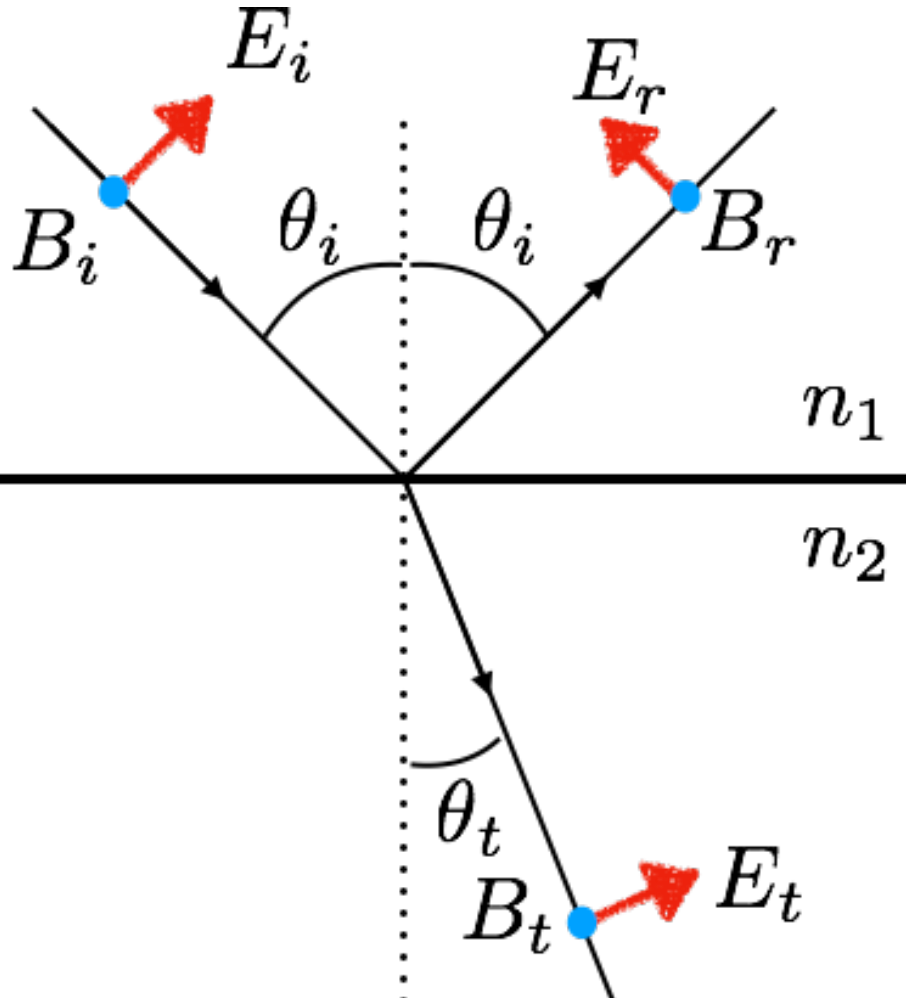
\includegraphics[width=0.2\textwidth]{Figures/p-polarization.png}
    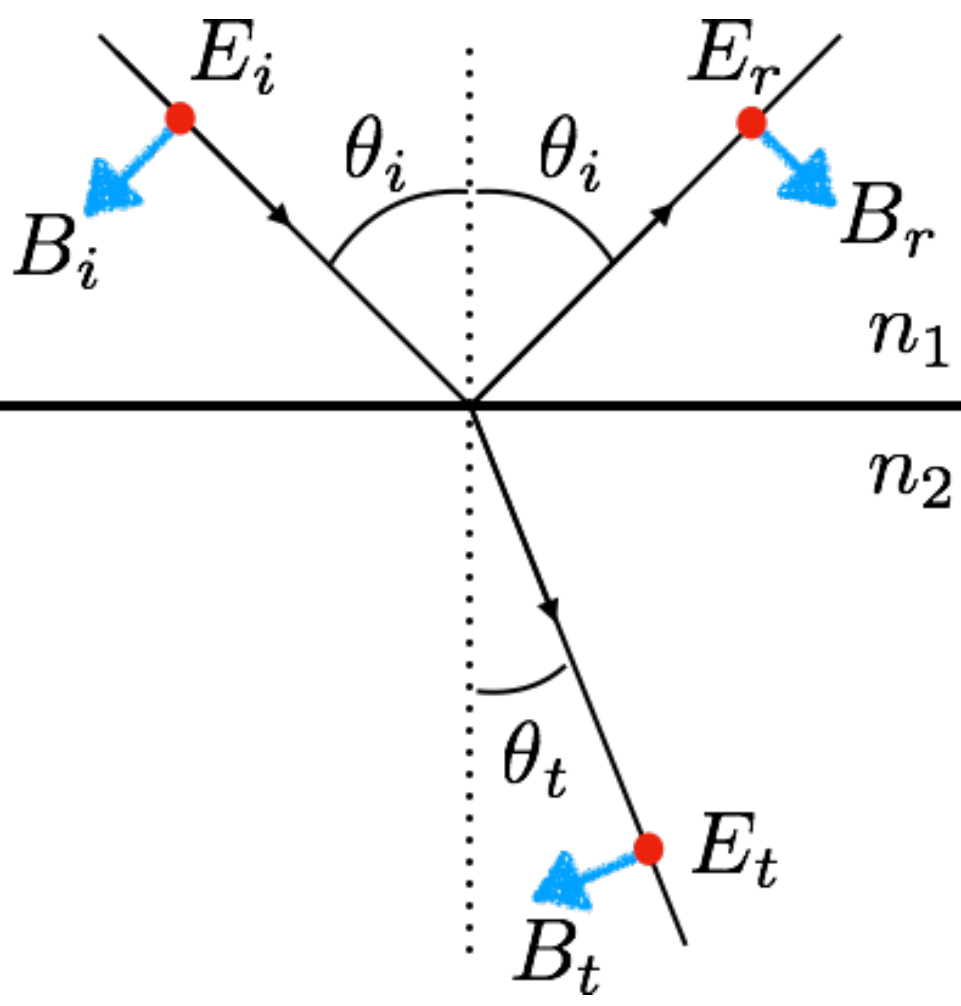
\includegraphics[width=0.2\textwidth]{Figures/s-polarization.png}
    \caption{Left: p-polarization, Right: s-polarization}
\end{figure}

Boundry conditions for amplitudes of plane waves across a planar interface:
\begin{align*}
    B_{\perp 1} = B_{\perp 2}
    \hspace{5pt} , \hspace{5pt}
    D_{\perp 1} = D_{\perp 2}
    \hspace{5pt} , \hspace{5pt}
    H_{\parallel 1} = H_{\parallel 2}
    \hspace{5pt} , \hspace{5pt}
    E_{\parallel 1} = E_{\parallel 2}
\end{align*}

With this we have: $E_i \cos(\theta_i) - E_r \cos(\theta_i) = E_t \cos(\theta_t)$
and $n_1 E_i + n_1 E_r = n_2 E_t$.

\subparagraph{Fresnel Equations}
\begin{enumerate}[]
    \item For p-polarization:
        \begin{align*}
            t_p &= \frac{E_t}{E_i} = \frac{2 n_1 \cos(\theta_i)}{n_2 \cos(\theta_i) + n_1 \cos(\theta_t)}
            \\
            r_p &= \frac{E_r}{E_i} = \frac{E_r}{E_i} = \frac{n_2 \cos(\theta_i) - n_1 \cos(\theta_t)}{n_2 \cos(\theta_i) + n_1 \cos(\theta_t)}
                = \frac{\tan(\theta_i - \theta_t)}{\tan(\theta_i + \theta_t)}
        \end{align*}
    \item For s-polarization:
        \begin{align*}
            t_s &= \frac{E_t}{E_i} = \frac{2 n_1 \cos(\theta_i)}{n_1 \cos(\theta_i) + n_2 \cos(\theta_t)}
            \\
            r_s &= \frac{E_r}{E_i} = \frac{n_1 \cos(\theta_i) - n_2 \cos(\theta_t)}{n_1 \cos(\theta_i) + n_2 \cos(\theta_t)}
        \end{align*}
\end{enumerate}


\paragraph{Brewster's Angle}

$r_p = 0 \Leftrightarrow \theta_i + \theta_t = \frac{\pi}{2}$. This special value
of $\theta_i$ is called Brewster's angle, labeled $\theta_B = \arctan(n_2/n_1)$.
For light waves incident at an angle of $\theta_B$, no p-polarized light can be
reflected. For s-polarized light, there is no incidence angle where there is no
zero reflectivity.


\subsection{Spectroscopy}

\paragraph{Grating Spectrometer}
Phase difference between the light reflecting off of two neighboring stips:
\begin{align*}
    \phi(\lambda) = k d \klammer{\sin(\theta_i) - \sin(\theta_j)}
    \hspace{10pt} , \ k = \frac{2 \pi}{\lambda}
\end{align*}
Contribution from $N$ strips:
\begin{align*}
    U &\propto \sum_{n=0}^{N-1} e^{i n \phi} = \frac{1 - e^{i N \phi}}{1 - e^{i \phi}}
    = e^{i(N-1)\phi/2} \frac{\sin\klammer{N \phi / 2}}{\sin(\phi/2)}
    \\
    I &\propto \abs{U}^2 \propto \frac{\sin^2 \klammer{N \phi / 2}}{\sin^2(\phi/2)}
\end{align*}
Maxima at $\phi/2 = m \pi$ with $m \in \Z$. Maximal value: $N^2$. Yields:
\begin{align*}
    \sin(\theta_i) - \sin(\theta_j) = \frac{2 \pi m}{d k} = \frac{m \lambda}{d}
\end{align*}
$m$ is the \fat{order of the maximum}. Condition for Minima:
\begin{align*}
    \frac{\phi_2}{2} = \klammer{m + \frac{1}{N}} \pi
\end{align*}
Combinint conditions:
\begin{align*}
    \phi_2 - \phi_1 &= \frac{2 \pi}{N}
    \\
    k_2 - k_1 &= \frac{2 \pi}{N d \klammer{\sin(\theta_i) - \sin(\theta_j)}}
    \\
    \Delta \nu &= \frac{c}{N d \klammer{\sin(\theta_i) - \sin(\theta_j)}}
\end{align*}


\paragraph{Interferometry}
Consider Michelson inferometer. Beamsplitter devides input beams evenly into two
parts of equal amplitude and phase and does the inverse of this on recombination.
Electric field on detector:
\begin{align*}
    U \propto \frac{1}{2} U_0 e^{2 i k d_1} + \frac{1}{2} U_0 e^{2 i k d_2}
    = \frac{U_0}{2} e^{2 i k d_1} \klammer{1+e^{2 i k x}}
\end{align*}
where $U_0$ is the input amplitude, $d_1$ and $d_2$ are the optical path lengths
and $x = d_2 - d_1$. With this:
\begin{align*}
    I \propto \frac{\abs{U_0}^2}{4} \klammer{2 + 2 \cos(2 k x)}
    \propto \frac{I_0}{2} \klammer{1+\cos(4 \pi x / \lambda)}
\end{align*}

The \fat{spectral density} $S(\nu)$ of a light source:
$S(\nu) d \nu$ is the power emitted by the light source between frequencies
$\nu$ and $\nu + d \nu$.
\begin{align*}
    I &\propto \int_0^\infty S(\nu) \klammer{1+\cos(4 \pi x / \lambda)} \ d \nu
    \\
    &\propto \int_0^\infty S(\nu) \ d \nu + \int_0^\infty S(\nu) \cos(4 \pi \nu x / s) \ d \nu
    \\
    &\propto \int_0^\infty S(\nu) \ d \nu + \frac{1}{2} \intii S(\abs{\nu}) e^{i 4 \pi \nu x / c} \ d \nu
\end{align*}
\begin{align*}
    S(\nu) &\propto \int_0^\infty \klammer{2 I(x) - I_0} \cos(4 \pi \nu x / c) \ d x
    \\
    &\sim \int_0^{x_{\text{max}}} \klammer{2 I(x) - I_0} \cos(4 \pi \nu x / c) \ d x
    \\
    &\sim \int_0^{x_{\text{max}}} \cos (4 \pi x \nu_0 / c) \cos(4 \pi x \nu / c) \ dx
    \\
    &\sim \text{sinc} \klammer{\frac{2 \pi (\nu - \nu_0) x_{\text{max}}}{c}}
        + \text{sinc} \klammer{\frac{2 \pi (\nu + \nu_0) x_{\text{max}}}{c}}
\end{align*}
This peaks at $\nu = \pm \nu_0$. Zeros closest to the maximum at $+\nu_0$ are at
\begin{align*}
    \nu - \nu_0 = \pm \frac{c}{2 x_{\text{max}}}
\end{align*}
Thus, according to Rayleigh criterion our spectrometer resolution is
\begin{align*}
    \frac{\Delta \nu}{\nu_0} = \frac{\lambda}{2 x_{\text{max}}}
    \hspace{10pt} \text{ or } \hspace{10pt}
    \delta \nu = \frac{c}{2 x_{\text{max}}}
\end{align*}

\paragraph{Fabry-Perot etalon}
Incomming light source: $A_0 e^{i(k x - \omega t)}$, $t$: transmission coefficient,
$r$: reflection coefficient. Transmitted field: $A_0 \cdot t$, reflected field:
$A_0 \cdot r \cdot e^{i \phi_r}$. Total field amplitude from all the paths:
\begin{align*}
    A &= A_0 t^2 e^{i k d} \sum_{n=0}^\infty r^{2n} e^{i n \phi}
    = A_0 t^2 e^{i k d} \cdot \frac{1}{1 - r^2 e^{i \phi}}
    \\
    \eta = \frac{\abs{A}^2}{\abs{A_0}^2} &= \frac{t^4}{\klammer{1 - r^2 e^{i \phi}} \klammer{1 - r^2 e^{-i \phi}}}
        = \frac{t^4}{1 + r^4 - 2 r^2 \cos(\phi)} 
    \\
    &= \frac{\klammer{1-R}^2}{(1-R)^2 + 2 R (1-\cos(\phi))}
        = \frac{1}{1 + \frac{4 R}{(1-R)^2} \sin^2 \klammer{\frac{\phi}{2}}}
    \\
    \eta = \frac{I_o}{I_i} &= \frac{1}{1+ \frac{4 R}{(1-R)^2} \sin^2 \klammer{2 \pi d / \lambda + \phi_r}}
\end{align*}
with $T = t^2$, $R = r^2$ and $t^2 + r^2 = 1$. $R$ is the reflectivity of the
mirror, $d$ the distance between the mirrors, and $\lambda$ is the wavelength
of the light, and $\phi_r$ is the phase picked up by the light when it reflects off
a mirror.
Wavelength resolution $\delta \nu$:
\begin{align*}
    \frac{d \lambda}{d \nu} = \frac{d}{d \nu} \klammer{\frac{c}{\nu}} = - \frac{c}{\nu^2}
    \hspace{10pt} \Rightarrow \hspace{10pt}
    \delta \lambda = \frac{c}{\nu^2} \delta \nu
\end{align*}



\section{Statistical Physics}

A single macrostate can be consistant with many microstates. A single microstate,
however, always specifies a single macrostate. A microstate contains all the
information about the macrostate, but not vice versa.

\paragraph{Fundamental postulate of statistical physics}
\textit{"For a closed system, every microstate which satisfies the global constraint is
equally likely to be occupied."} "closed system" = system that does not exchange
matter with the outside but it can exchange energy, "global constraint" = system
has a particular set of values for global variables such as the particle number,
volume, energy, etc. Systems that fulfil this postulate are said to be in a
\fat{thermodynamic equilibrium}. Further postulates: \textit{"Over a sufficiently
long period of time, a system will sample every microstate compatible with the
global constraints with equal property."}, \textit{"The macrostate occupied in
thermodynamic equilibrium is the one with the largest number of microstates."}

\paragraph{Variance}
$\Delta z = \sqrt{\langle z^2 \rangle - \langle z \rangle^2}$. 
The factorial width $\Delta z / \langle z \rangle$ decreases as $1/\sqrt{N}$.

\paragraph{Ideal gas law}
$p V = N k_B T = N m \langle v_x^2 \rangle$

\paragraph{Temperature}
For an isolated system with two chambers with energies $U_i$ and numbers of
particles $N_i$, we have:
\begin{align*}
    \frac{1}{\Omega_1} \klammer{\frac{\partial \Omega_1}{\partial U_1}}_{N_1}
    = \frac{1}{\Omega_2} \klammer{\frac{\partial \Omega_2}{\partial U_2}}_{N_2}
    &\Leftrightarrow
    \klammer{\frac{\partial}{\partial U_1} \ln (\Omega_1)}_{N_1}
    = \klammer{\frac{\partial}{\partial U_2} \ln (\Omega_2)}_{N_2}
    \\
    \klammer{\frac{\partial \sigma_1}{\partial U_1}}_{N_1}
    &= \klammer{\frac{\partial \sigma_2}{\partial U_2}}_{N_2}
\end{align*}
Where $\Omega_i$ is the number of microstates corresponding to the macrostates
specified by $N_i$ and $U_i$. The total number of microstates is given by
$\Omega(N_1 , N_2 , U_1 , U_2) = \Omega(N_1 , U_1) \cdot \Omega(N_2 , U_2)$.
We define $\sigma = \ln (\Omega)$. This relation between two systems must hold, 
when thermodynamic equilibrium is reached. Temperature is defined as
\begin{align*}
    \frac{1}{T} = k_B \klammer{\frac{\partial \sigma}{\partial U}}_{N,V}
\end{align*}
Definitions: $\tau = k_B T$, $\beta = 1 / \tau = 1 / k_B T$.

\paragraph{Entropy}
$S = k_B \sigma = k_b \ln (\Omega) = - k_B \sum_s p_s \log(p_s) =
\frac{\partial}{\partial T} \klammer{k_B T \ln(Z)}$

\paragraph{Boltzmann factor and partition function}
Probability of finding a system in thermal equilibrium in a microstate with energy
$\epsilon$ is proportional to $e^{-\beta \epsilon}$, called Boltzmann factor.
Absolute probability of finding the system in a microstate with energy $\epsilon$
\begin{align*}
    P(\epsilon) = \frac{e^{-\beta \epsilon}}{Z}
    \hspace{10pt} , \hspace{10pt}
    Z = \sum_s e^{-\beta \epsilon_s}
    \hspace{10pt} , \hspace{10pt}
    U = \langle \epsilon \rangle - \frac{\partial}{\partial \beta} (\ln (Z))
\end{align*}
where $Z$ is called \fat{partition function}. $U$ is the average energy of the system.
The continuous form of the partition function is:
\begin{align*}
    Z
    = \sum_{E_s} \Omega (E_s) e^{-\beta E_s}
    = \int_0^\infty f(E) e^{-\beta E} \ d E
\end{align*}

\paragraph{Partition function}
Partition function for a single particle in $3D$:
\begin{align*}
    Z_{sp}
    = \frac{V}{h^3} \klammer{\frac{2 \pi m}{\beta}}^{3/2}
    = V \klammer{\frac{2 \pi m k_B T}{h^2}}^{3/2}
\end{align*}
where $V$ = volume and $h$ = Plank constant. For \underline{distinguishable}
particles: $Z_D = Z_{sp}^N$.
For \underline{indistinguishable particles}: $Z_I = \frac{1}{N!} Z_{sp}^N$.

\paragraph{Heat Capacity}
$\frac{1}{C} = \frac{\partial T}{\partial E} \Leftrightarrow
C = \frac{\partial E}{\partial T}$

\paragraph{Average Energy}
$\langle E^k \rangle = \frac{1}{Z} \int_0^\infty E^k p(E) \ dE$

\paragraph{Variance}
$(\Delta E)^2 = \langle E^2 \rangle - \langle E \rangle^2 = \frac{\partial^2 \log(Z)}{\partial \beta^2}$

\paragraph{Equipartition Theorem}
\textit{Each term in the energy that is quadratic in some coordinate contributes
$k_B T / 2$ to the average energy per particle.}

\paragraph{Gases of polyatomic molecules}
Internal degrees of freedom also contribute to the energy $U$. Each distinguishable,
independent rotation axis gives \underline{one} extra quadratic term to the
microstate energy. Each vibration mode gives \underline{two} such terms: one for
the displacement, and one for the momentum.

\paragraph{Maxwell-Boltzmann distribution}
Total number of microstates with momentum magnitude between $p$ and $p + dp$ is
$g(p) dp = \frac{4 \pi V p^2 dp}{h^3}$ with $g(p)$ the multiplicity function.
Probability of finding a particle with momentum between $p$ and $p+dp$ as
$P(p) dp = \frac{4 \pi V p^2 dp}{h^3} \cdot \frac{e^{-\beta p^2 /2m}}{Z_{sp}}$.
Expected number of particles in the gas with speeds between $v$ and $v+dv$:
\begin{align*}
    n(v) dv = 4 \pi N v^2 dv \klammer{\frac{m}{2 \pi k_B T}}^{3/2} e^{-m v^2 / 2 k_B T}
\end{align*}
Average speed of a particle in an ideal gas: $\langle v \rangle =
\frac{\int_0^\infty v n(v) dv}{N} = \sqrt{\frac{8 k_B T}{\pi m}}$.
Most probable speed (maximum of distribution): $v_{max} = \sqrt{\frac{2 k_B T}{m}}$.
\underline{Important}: speed $v$ is the \textit{magnitude} of the particles speed.
For $v_x$: $\langle v_x \rangle = 0$, $\langle v_x^2 \rangle = \frac{k_B T}{m}$

\paragraph{Blackbody Radiation}
A blackbody is an object that absorbs all light that hits it. In order to stay
in thermal equilibrium with its surrounding, the blackbody also needs to emit
light. Consider a rectangular box as a blackbody. Then the $1D$-solution to the
waveequation is given as: $E(x,t) = \vec{E}_0 \sin(k_x x) e^{i \omega t}$,
where $k_x = \frac{n \pi}{L_x}$ with $n=1,2,\dots$ and $L_x$ the length of the
box in $x$-direction. In $3D$:
\begin{align*}
    \vec{E}(x,y,z,t) = \begin{pmatrix}
        E_{0,x} \cos(k_x x) \sin(k_y y) \sin(k_z z) \\
        E_{0,y} \sin(k_x x) \cos(k_y y) \sin(k_z z) \\
        E_{0,z} \sin(k_x x) \sin(k_y y) \cos(k_z z)
    \end{pmatrix} \cdot e^{i \omega t}
\end{align*}
$\vec{k} = \klammer{\frac{n_x \pi}{L_x} , \frac{n_y \pi}{L_y} , \frac{n_z \pi}{L_z}}$,
$n_x,n_y,n_z \in \N$, $\omega = c \cdot \abs{\vec{k}}$, $\vec{E}_{0} \cdot k = 0$.
Number of modes with wavevector magnitudes between $k$ and $k+dk$ is then given by
\begin{align*}
    g(k) \ dk = \frac{V}{\pi^2} k^2 \ dk
    \hspace{10pt} , \hspace{10pt}
    g(\nu) \ d \nu = \frac{8 \pi V}{c^3} \nu^2 \ d \nu
\end{align*}

\paragraph{Rayleigh-Jeans Law}
Energy density of the electromagnetic field:
\begin{align*}
    u = \frac{1}{2} \klammer{\epsilonnull E^2 + \frac{1}{\munull} B^2}
\end{align*}
Each allowed mode with wavevector $\vec{k}$ and polarization $\vec{\epsilon}$ of the
EM field inside the cavity with an $E$-field amplitude $E_{\vec{k},\vec{\epsilon}}$
and magnetic field amplitude $B_{\vec{k},\vec{\epsilon}}$ has an energy
\begin{align*}
    \epsilon_{\vec{k},\vec{\epsilon}} = \frac{V}{4} \klammer{\epsilonnull E_{\vec{k},\vec{\epsilon}}^2 + \frac{1}{\munull} B_{\vec{k},\vec{\epsilon}}^2}^2
\end{align*}
Total EM energy: $\epsilon = \sum_{\vec{k},\vec{\epsilon}} \epsilon_{\vec{k},\vec{\epsilon}}$ ,
$\langle \epsilon_{\vec{k},\vec{\epsilon}} \rangle = k_B T$,
energy density inside the box for all modes within a cycle frequency between $\nu$
and $\nu + d \nu$ is then
\begin{align*}
    \rho(\nu) \ d \nu &= k_B T \cdot \frac{g(\nu) \ d \nu}{V} = k_B T \cdot \frac{8 \pi \nu^2}{c^3} \ d \nu
    \\
    \rho(\omega) \ d \omega &= k_B T \cdot \frac{\omega^2}{\pi^2 c^3} \ d \omega
\end{align*}
Problem: if $\omega \rightarrow \infty$, then $\rho(\omega) \rightarrow \infty$.

\paragraph{The Planck Distribution}
Idea to solve ultraviolet catastrophe: only discrete values of energies are
allowed. Assumption: energies are multiples of $\hbar \omega$. Then the
partition function becomes:
\begin{align*}
    Z = \sum_{n=0}^\infty e^{-\beta n \hbar \omega} = \frac{1}{1 - e^{-\beta \hbar \omega}}
\end{align*}
The average energy is then:
\begin{align*}
    \langle \epsilon \rangle = - \frac{\partial}{\partial \beta} (\ln(Z))
    = \frac{\hbar \omega}{e^{\beta \hbar \omega} - 1}
    \approx k_B T \ \text{ (if } k_b T \gg \hbar \omega )
\end{align*}
Now the energy distribution (Plank distribution ) is given by
\begin{align*}
    \rho(\omega) \ d \omega &= \frac{\hbar \omega^3}{\pi^2 c^3} \frac{d \omega}{e^{\beta \hbar \omega} -1}
    \\
    \rho(\nu) &= \frac{\langle E(\nu) \rangle g(\nu)}{V^2} \ \text{(If 2D), if 1D: V}
\end{align*}
Total EM energy density: (Stefan-Boltzmann Law)
\begin{align*}
    u = \int_0^\infty \rho(\nu) \ d \nu= \frac{U}{V} =
    \underbrace{\frac{8 \pi^5 k_B^4}{15 h^3 c^3}}_{:= a} T^4
    = a T^4
\end{align*}
Emitted power per unit area of the blackbody surface
\begin{align*}
    j(T) = \underbrace{\frac{a c}{4}}_{:= \sigma} T^4  
    = \sigma T^4
\end{align*}
$\sigma$ is called Stefan's constant.


\section{Atoms}

\paragraph{Elements}
${^A_Z}G$: $A$ is the mass of the atom, $G$ is the symbol of the element and $Z$
is the atomic number (number of protons).

\paragraph{Mass spectrometer}
$\vec{E} = E \vec{e}_y$ , $\vec{B} = B \vec{e}_y$ , $\vec{v} = v \vec{e}_z$ ,
$\vec{F} = q \klammer{\vec{E} + \vec{v} \times \vec{B}}$. Thus
$m \frac{d^2 y}{d t^2} = q E \Rightarrow y = \frac{q E t^2}{2 m}$ and
$m \frac{d^2 x}{d t^2} = - q B v \Rightarrow x = - \frac{q B v t^2}{2 m}$.
Since $t = l/v$ we obtain $y = \frac{m}{q} \frac{2 E x^2}{B^2 l^2}$. Where $l$ is
the length of the condensator (interaction length). This is a parabola. Depending
on the ratio $m/q$ the particle will land somewhere else.

\paragraph{Scattering}
Assume we scatter atoms with radius $r_1$ and $r_2$, then they can't get
closer than $r_1 + r_2$. Then the \fat{scattering cross section} is
$\sigma = \pi (r_1 + r_2)^2$. The \fat{flux} is defines as
$F = \frac{\Delta N_p}{A \Delta t}$. Rate of hitting objects is
$R = F \sigma$. Using a \textit{collection} of atoms as target:
probability of two atoms lining up is small, rate of interactions is then
$R = F \sigma N_A$ with $N_A$ the number of atoms interacting with the beam.
Assume atoms have a uniform density $n$ within the volume. Probability that
a single incident atom will get scattered: $P_S = n \sigma d x$.
Change in number of atoms in the beam is $d N = - N \sigma n dx$. After a
distance $x$, the number of remaining particles is $N(x) = N(0) e^{-n \sigma x}$.
Number of particles over a time $T$ through the entire cylinder is then
$N(L) = N(0) e^{- \sigma n L}$, thus: $\sigma = \frac{\ln \klammer{\frac{N(p)}{N(L)}}}{n L}$.

\paragraph{Rutherford Scattering}
Shooting $\alpha$ particles at atom. Coulomb force acting:
$\vec{F} = \frac{k}{r^2} \hat{r}$ with $k = \frac{2 Z e^2}{4 \pi \epsilon_0}$
with charge electron charge $e$ and atomic number $Z$. Since force is central,
angular momentum needs to be conserved, resulting in $m v_0 b = m \dot{\phi} r^2
\Rightarrow \frac{1}{r^2} = \frac{\dot{\phi}}{v_0 b} \Rightarrow \vec{F} =
\frac{k \dot{\phi}}{v_0 b} \hat{r} \Rightarrow F_{\perp} = \frac{k \dot{\phi}}{v_0 b}
\sin(\phi) \Rightarrow m \dot{v}_{\perp} = \frac{k \dot{\phi}}{v_0 b} \sin(\phi)$
Integrate this over a long period of time, $t_1$ long before interaction,
$t_2$ long after interaction. At $t_1$: $v_\perp = 0$. At $t_2$:
$v_\perp (t_2) = v_0 \sin(\theta)$, $\phi = \phi_2 = \pi - \theta$, so:
$\int_{t_1}^{t_2} \frac{d v_\perp}{dt} dt = \int_{t_1}^{t_2} \frac{k}{m v_0 b} \sin(\phi) \frac{d \phi}{dt} dt$
resulting in $\int_0^{v_0 \sin(\theta)} d v_\perp = \int_0^{\pi-\theta} \frac{k \sin(\phi)}{m v_0 b} d \phi$
resulting in $v_0 \sin(\theta) = \frac{k}{m v_0 b} \klammer{1 + \cos(\theta)}$
meaning $b = \frac{k}{m v_0^2} \cot \klammer{\frac{\theta}{2}}$.
Now the goal is to find the distribution of particles over deflection angle.
If we have a flux of particles $F = R/A$, then $d R = F \cdot 2 \pi b \ db
= \pi F \klammer{\frac{k}{m v_0^2}}^2 \frac{\cos(\theta/2)}{\sin^3(\theta/2)} d \theta$.
The differential \fat{solid angle} is defined as $d \Omega = d A_{det} / r_{det}^2$,
with $d A_{det}$ the projection area of the detector and $r_{det}$ the distance
to the detector. $d \Omega = \sin(\theta) d \theta d \gamma$ with $d \gamma$ the
azimuthal angle interval giving the size along the direction orthogonal to $d \theta$.
So we obtain $d R = \frac{F}{4} \klammer{\frac{k}{m v_0^2}}^2 \frac{1}{\sin^4(\theta/2)} d \Omega$.
Differential cross section: $d R = F d \sigma \Rightarrow d \sigma =
\frac{1}{4} \klammer{\frac{k}{m v_0^2}}^2 \frac{1}{\sin^4(\theta/2)} d \Omega$.
$d \sigma$ is called \textit{Rutherford's differential cross section scattering
formula}.

\vspace{1\baselineskip}

\fat{$d \dot{N} = F d \sigma$} with $dN$ the change in the rate of particles
through some differential area $d \sigma$ and $F$ the flux.

\vspace{1\baselineskip}

$b = \frac{k}{m v_0^2} \cot(\theta/2)$ for $ \sim 1 \mathrm{fm} \ll b \ll r_a$

\vspace{1\baselineskip}

$d \Omega = 2 \pi \sin(\theta) d \theta$


\section{Photons and Particle-Wave Duality}

\paragraph{The Photoelectric Effect}
Under some circumstances, light causes negative charges (electrons) to be ejected
from a metal plate. Will not work if the plate has too much positive charge or if
the frequencies of the light are too low.
For each frequency of light there is a different voltage $V_{max}$ at which
electrons are ejected from the emitter plate are no longer able to reach the
the collector plate. We have $E_{kin}^{max} = e V_{max}$, and
$E_{max} = h \nu - \Phi$ with $\Phi$ the work function. Thus, \textit{The energy
contained in light with frequency $\nu$ can be absorbed only in multiples of
$h \nu$. This quantum of light is called a photon}.

\paragraph{The Inverse Photoelectric Effect and X-Rays}
Take an energetic free electron and bring it into a metal, thereby producing a
photon. The maximum frequency $\nu$ of photons emitted in this way is given by
the kinetic energy $E_{kin} = e V_0$ of the electrons that hit the anode, by the
relation $h \nu_{max} = e V_0 + \Phi$, where $\Phi$ is the work function.
In practice $\Phi \ll e V_0$, so $\nu_{max} = e V_0 / h$ and $\lambda_{min} =
h c / e V_0$.

\subsection{Scattering of photons with atoms}

% \paragraph{Rayleigh scattering}
% Photon-atom interaction. Elastic scattering of a photon with an atom or molecule.
% Elastic means, frequency of the photon does not change. If an electric field is
% present, nucleus and electron cloud shift in opposite directions. Separation is result
% of balance of forces from electric field $\vec{F}_{field} = -q \vec{E}$ versus
% attractive bonding interaction between nucleus and electrons, which can be approximated
% with Hook's Law $\vec{F}_{bond} = - k \vec{x}$. So, $m \frac{d^2 x}{d t^2} = - q E - k x$. 
% For light wave with angular frequency $\omega$, electric field oscillates as
% $E = E_0 \cos(\omega t)$, resulting in $\frac{d^2 x}{d t^2} + \frac{k}{m} x =
% - \frac{q}{m} E_0 \cos(\omega t)$. Define $\omega_0 = \sqrt{k/m}$ and use ansatz
% $x(t) = x_0 \cos(\omega t)$ with $x_0 = \frac{q E_0}{m (\omega^2 - \omega_0^2)}$.
% Harmonic motion of electon results in an oscillating dipole moment.
% Emitted electric field: $E_{emitted} \propto x_0 \cos(\omega t)$.
% Intensity emitted: $I_{emitted} \propto \langle \abs{E_{emitted}}^2 \rangle
% \propto \frac{q^2 E_0^2 \omega^4}{m^2 (\omega^2 - \omega_0^2)^2}$.
% This implies that the interaction of light field with an atom will result in the
% reemission of light from the atom as a new point source of light.

\subparagraph{X-Ray diffraction}
Constructive interference occurs if the optical path
length of the two paths differ by an integer multiple of the x-ray wavelength
$\lambda$. This results in the \fat{Bragg condition} $2 d \sin(\theta) = n \lambda$ with
$d$ the distance between planes of atoms. 

\paragraph{Compton Scattering}
Inelastic scattering, meaning, scattered light has a different energy
than the incident light. Consider photons as particles with energy $E = h \nu$
and momentum $p = E / c = h \nu / c = h / \lambda$. Consider interaction of a
single photon with an electron. Assume, electron initially at rest and photon moves
along positive $x$-direction. Let $\theta$ be the deflection angle of the photon
and $\phi$ be the deflection angle of the electron (with respect to the $x$-axis).
Goal: study relation between $\theta$ and $\Delta \lambda$ of the photon.
Conservation conditions yield:
$h \nu + m_e c^2 = h \nu' + \sqrt{m_e^2 c^4 + p^2 c^2}$,
$\frac{h \nu}{c} + 0 = \frac{h \nu'}{c} \cos(\theta) + p \cos(\phi)$
and $0 + 0 = \frac{h \nu'}{c} \sin(\theta) - p \sin(\phi)$. Thus:
$p^2 \cos^2 (\phi) = \frac{h^2}{c^2} (\nu - \nu' \cos(\theta))^2$,
$p^2 \sin^2 (\phi) = \frac{h^2 (\nu')^2}{c^2} \sin^2(\theta)$
$\Rightarrow p^2 c^2 = h^2 \klammer{\nu^2 - 2 \nu \nu' \cos(\theta) + (\nu')^2
\cos^2(\theta) + (\nu')^2 \sin^2(\theta)} = h^2 (\nu-\nu')^2 + 2 h^2 \nu \nu' (1-\cos(\theta))
= \klammer{h(\nu - \nu') + m_e c^2}^2 - m_e^2 c^4
= h^2 (\nu - \nu')^2 + 2 h (\nu - \nu') m_e c^2$. Further
$h \nu \nu' (1-\cos(\theta)) = (\nu - \nu') m_e c^2$
$\Rightarrow \Delta \nu = \frac{h \nu \nu'}{m_e c^2} (1-\cos(\theta))$.
Therefore:
$\Delta \lambda = \frac{c \Delta \nu}{\nu \nu'}
= \lambda_c (1-\cos(\theta))$ with $\lambda_c = \frac{h}{m_e c}$
the so called \fat{Compton wavelength}.


\subsection{Matter Waves}

\paragraph{De Broglie Wavelength}
$\lambda_{dB} = h / p = \frac{h}{\sqrt{2 m_e E_{kin}}}$ with $p$ the momentum of
the massiv particle. Equivalent: $p = \hbar k_{dB}$. Constructive interference: $d \sin(\phi) = n \lambda_{dB}$
with $d$ the distance between atoms, $n$ the order of the maximum and $\phi$ the
deflection angle.

$\langle E_{kin} \rangle = \frac{p^2}{2m} = \frac{3}{2} k_B T
\Rightarrow \lambda_{dB} = \frac{h}{\sqrt{3 m k_B T}}$

% \paragraph{Wavepackets}
% Superposition of waves for stationary wave:
% $\psi(x,t) = \int_{k_0 - \Delta k}^{k_0 + \Delta k} A e^{i (k x - \omega(k) t)} \ dk$
% For light: $\omega_{light} (k) = c k = E_{photon} / \hbar$. For matter waves:
% $\omega(k) = E_{kin} / \hbar$. For non relativistic particles:
% $\omega(k) = \frac{p^2}{2 m \hbar} = \frac{\hbar k^2}{2 m}$. If wavepackets only
% contain wavevectors very close to an average value $k_0$:
% $\omega(k) \approx \frac{\hbar k_0^2}{2 m} + \frac{\hbar k_0}{m} (k - k_0)$.
% Define $\omega_0 \equiv \frac{\hbar k_0^2}{2 m}$. Now:
% $\psi(x,t) \approx 2 A \Delta k e^{i(k_0 x - \omega_0 t)} \text{sinc}
% \eckigeklammer{\Delta k \klammer{x - \frac{\hbar k_0 t}{m}}}$. Peak of envelope
% of $\psi$ in $x$ is at $x_{max} = \frac{\hbar k_0 t}{m}$. \fat{Group velocity}:
% $\frac{d x_{max}}{dt} = \frac{\hbar k_0}{m} = \frac{p_0}{m} = v_0$. Width of
% envelope: $\Delta x = \frac{2 \pi}{\Delta k} = \frac{2 \pi \hbar}{\Delta p}$.
% Thus $\Delta x \Delta p = h$.

% \subparagraph{Physical meaning}
% The function $\psi(x,t)$ can be interpreted as giving the probability $P(x,t) dx$
% to find a particle at a position between $x$ and $x + dx$ at a time $t$ via
% $P(x,t) dx = \abs{\psi(x,t)}^2 dx$. Normalization condition:
% $\intii P(x,t) dx = 1$.

% \paragraph{Heisenberg Uncertainty Principle}
% % If $\Delta p_x$ and $\Delta x$ are standard deviations of the momentum and position,
% % then $\Delta p_x \Delta x \geq \frac{h}{2}$. This means, position and momentum
% % uncertainties of a particle along one axis are never known simultaneously to
% % arbitrary precision.
% $\Delta p_x \Delta x \geq \frac{h}{2}$


\section{Quantum Mechanics}

\paragraph{Heisenberg Uncertainty Principle}
% If $\Delta p_x$ and $\Delta x$ are standard deviations of the momentum and position,
% then $\Delta p_x \Delta x \geq \frac{h}{2}$. This means, position and momentum
% uncertainties of a particle along one axis are never known simultaneously to
% arbitrary precision.
$\Delta p_x \Delta x \geq \frac{h}{2}$

% \subsection{Wavefunction}
% The state of every quantum system can be completely described by a complex valued
% function $\psi(x,t)$ called the wavefunction. The probability of finding a particle
% between $x$ and $x+dx$ is $P(x,t) dx = \abs{\psi(x,t)}^2 dx = \overline{\psi(x,t)}
% \psi(x,t) dx$. Normalization $\intii \abs{\psi(x,t)}^2 dx = 1$.

% \subsection{Basis Sets of Functions}

% \paragraph{Fourier Series}
% $\psi(x) = \sum_{n=-\infty}^\infty \psi_n e^{i 2 \pi n x / L}$ with
% $x \in (-L/2,L/2)$ and $\psi_n = \frac{1}{L} \int_{-L/2}^{L/2} \psi(x) e^{-2\pi i n x / L} dx$

% \paragraph{Discrete Bases}
% Suppose we have a set of orthogonal functions $\phi_n(x)$. Meaning:
% $\int_D \overline{\phi_m(x)} \phi_n(x) dx = \delta_{mn}$ with $D$ the domain
% of the set of functions. Such a set is called a \fat{complete orthonormal basis}
% if any function $\psi(x)$ defined on $D$ can be written as
% $\psi(x) = \sum_n \psi_n \phi_n(x)$ with $\psi_n = \int_D \overline{\phi_n(x)}
% \psi(x) dx$ inserting back yields $\sum_n \overline{\phi_n(x')} \phi_n(x) = \delta(x-x')$.
% This is called the \fat{completeness condition} and must be sstisfied for the $\phi_n(x)$
% in order to be a complete basis.
% Properties of the delta function: $\delta(x) = 0 \ \forall x \neq 0$, $\int_{-a}^a
% \delta(x) dx = 1$ for any $a>0$, $\delta(ax) = \frac{1}{\abs{a}} \delta(x) \
% \forall a \in \R$ and $\int \delta(x-x') g(x') dx' = g(x)$.

% \paragraph{Continuous Bases}
% Continuous variable $\alpha \in \R$, basis vectors $\phi(\alpha,x)$. Orthogonality:
% $\int \overline{\phi(\alpha,x)} \phi(\beta,x) dx = \delta(\alpha-\beta)$.
% Completeness condition: $\int \overline{\phi(\alpha,x)} \phi(\alpha,x) d \alpha 
% = \delta(x-x')$. Then $\psi(x) = \int \tilde{\psi}(\alpha) \phi(\alpha,x) d \alpha$
% with $\tilde{\psi}(\alpha) = \int \overline{\phi(\alpha,x)} \psi(x) dx$.

\subsection{Operators}
\fat{Observables}: observable property of a system. Observables are represented by
\fat{operators}. Suppose we have a wavefunction $\psi(x,t) = A e^{i(kx-\omega t)}$
with $p = \hbar k$ and $E = \hbar \omega$. The \fat{Eigenstate} is the physical
state represented by the eigenfunction.
\begin{enumerate}[]
    \item \fat{Position Oberator}: $\hat{x} = x$ or $-i \hbar \frac{\partial}{\partial p}$
    \item \fat{Momentum operator}: $\hat{p} = -i \hbar \frac{\partial}{\partial x}$ of $p$
    \item \fat{Energy operator}: $\hat{E} = i \hbar \frac{\partial}{\partial t}$
\end{enumerate}
% All physical observables are associated with Hermetian operators. The eigenvalue
% of these operators give the result of all possible measurements of the
% observable.

\subsection{Operator Representation}
% Any wavefunction can be expressed as the sum of eigenfunctionf of an observable
% operator. If in addition the eigenvalue of all the eigenfunctions are distinct,
% then it is possible to represent the wavefunction as a function of the eigenvalues
% of the operator. Eigenfunctions of position operator are $\delta(x-\alpha)$
% with eigenvalue $\alpha$. Thus, the wavefunction is representable as
% $\psi(\alpha,t) = \int \delta(x-\alpha) \psi(x,t) dx$ and hence $\psi(x,t)$ is
% the position operator representation of the wavefunction.

\paragraph{Momentum Basis}
We can write wave functions $\psi(x,t)$ in the momentum basis $\phi_p(x) =
\frac{1}{\sqrt{2 \pi \hbar}} e^{i p x / \hbar}$ with the following relation.
$\tilde{\psi}(p,t) = \frac{1}{\sqrt{2 \pi \hbar}} \int \psi(x,t) e^{-i p x / \hbar} dx$.
% Probability of measuring the momentum of the system between $p$ and $p+dp$:
% $P(p) dp = \abs{\tilde{\psi}(p,t)}^2 dp$.
Backtransformation:
$\psi(x,t) = \frac{1}{\sqrt{2 \pi \hbar}} \int \psi(p,t) e^{i p x / \hbar} dp$.

% \paragraph{Spectral Theorem}
% The eigenfunction of an operator $\hat{O}$ representing an observable form a
% complete, orthonormal basis.

\subsection{Hilbert Space and Dirac Notation}
% Column vector: $| S(t) \rangle$, row vector: $\langle S(t) |$.
% We find the representation of a state vector in a particular basis if we take the
% inner product with the basis states. In \fat{Dirac notation}:
% $\psi(x,t) = \langle x | S(t) \rangle$ where $\langle x |$ are the eigenstates
% of the position operator $\hat{x}$. We call $\langle \ | \ \rangle$ a
% \fat{bracket}, $\langle \ |$ the bra and $| \ \rangle$ the ket. Similarly
% $\tilde{\psi}(p,t) = \langle p | S(t) \rangle$. We can write $| S(t) \rangle$
% in different ways:
% \begin{align*}
%     | S(t) \rangle &= \int \psi(x,t) | x \rangle dx
%         = \int \psi(x,t) \delta(x-y) dx
%     \\
%     &= \int \tilde{\psi}(p,t) | p \rangle dp
%         = \int \tilde{\psi}(p,t) \frac{e^{i p x / \hbar}}{\sqrt{2 \pi \hbar}} dp
%     \\
%     &= \sum_n c_n (t) | \phi_n \rangle 
%         = \sum_n c_n (t) \phi_n (x)
%     \\
%     c_n (t) &= \langle e_n | S(t) \rangle 
%         = \intii \overline{\phi_n(x)} \psi(x,t) dx
% \end{align*}
% Orthogonality condition: $\langle \phi_n | \phi_m \rangle = \delta_{mn}$.
% Operators can be written as $\hat{O} = | \alpha \rangle \langle \beta |$.
\fat{Identity operator}: For a discrete basis: $\hat{I} = \sum_n | \phi_n \rangle \langle \phi_n |$,
for a continuous basis: $\int | \phi(\alpha) \rangle \langle \phi(\alpha) | d \alpha = 1$.
For continuous basis: $\langle \phi(\alpha) | \phi(\beta) \rangle = \delta (\alpha - \beta)$.

\subsection{Quantum Measurements}

% \paragraph{Spectral Theorem}
% The eigenstates of an observable operator $\hat{O}$ form a complete basis
% $\geschwungeneklammer{| o_n \rangle}$ (for discrete bases) or
% $\geschwungeneklammer{| o(\alpha) \rangle}$ (for a continuous basis).
% So any state $| \psi \rangle$ can be written as
% $| \psi \rangle = \sum_n c_n (t) | o_n \rangle$ or
% $| \psi \rangle = \int \psi(\alpha,t) | o(\alpha) \rangle d \alpha$

% \vspace{1\baselineskip}

If we make a measurement of the observable, we will get one eigenvalue as a result.
For a discrete basis, the probability of getting the result $o_n$ is
$\abs{\langle o_n | \psi \rangle}^2 = \abs{c_n}^2$.
After getting this result, the state of the system becomes $| o_n \rangle$.
This is also called \fat{collapse} of \fat{projection} of $| \psi \rangle$
into $| o_n \rangle$.
For a continuous basis, the probability of getting a result between $o(\alpha)$
and $o(\alpha + d \alpha)$ is $\abs{\langle o(\alpha) | \psi \rangle}^2 d \alpha
= \abs{\psi(\alpha,t)}^2 d \alpha$

\subsection{Operator Commutation}
If two different operators share the same eigenstate, then particles in those states
have simultanously definite values for both of those observables.
Suppose we have two observables that share the same eigenstate $\psi$, then
$\hat{O} \psi = O \psi$ and $\hat{Q} \psi = Q \psi$ with $O$ and $Q$ the corresponding
eigenvalues. We define the \fat{commutator} $\eckigeklammer{\hat{Q},\hat{O}} \equiv
\hat{Q} \hat{O} - \hat{O} \hat{Q}$. \textit{Two observable operators can share the
same eigenstates if and only if $\eckigeklammer{\hat{Q},\hat{O}} =
\eckigeklammer{\hat{O},\hat{Q}} = 0$.}
The \fat{anticommutator} is defined as
$\geschwungeneklammer{\hat{O},\hat{Q}} = \hat{O} \hat{Q} + \hat{Q} \hat{O}$

\paragraph{Identities}
$\eckigeklammer{\hat{A},c} = 0$ , $\eckigeklammer{\hat{A},\hat{A}} = 0$ ,
$\eckigeklammer{\hat{A},\hat{B}} = - \eckigeklammer{\hat{B},\hat{A}}$ ,
$\eckigeklammer{\hat{A},\sum_n c_n \hat{A}^n} = 0$ ,
$\eckigeklammer{c \hat{A},\hat{B}} = \eckigeklammer{\hat{A},c B} = c \eckigeklammer{\hat{A},\hat{B}}$ ,
$\eckigeklammer{\hat{A},\hat{B} \pm \hat{C}} = \eckigeklammer{\hat{A},\hat{B}} \pm \eckigeklammer{\hat{A},\hat{C}}$ ,
$\eckigeklammer{\hat{A} \hat{B} , \hat{C}} = \hat{A} \eckigeklammer{\hat{B},\hat{C}} + \eckigeklammer{\hat{A},\hat{C}} \hat{B}$ ,
$\eckigeklammer{\hat{A} , \hat{B} \hat{C}} = \hat{B} \eckigeklammer{\hat{A},\hat{C}} + \eckigeklammer{\hat{A},\hat{B}} \hat{C}$

\paragraph{Important commutators}
$\eckigeklammer{\hat{x},\hat{p}} = i \hbar$, in 3D: $\eckigeklammer{x_i,p_j} = i \hbar \delta_{ij}$
and $\eckigeklammer{x_i,x_j} = 0$

\subsection{Measurement for degenerate observables}
\fat{Degeneracy} is the property that  an observable operator has orthonormal
eigenfunctions with the same eigenstate.

Suppose we have a wavefunction $\psi(x)$ that describes a quantum state. This
wavefunction can be decomposed into a basis of orthonormal eigenfunctions $\phi_n(x)$
of an observables $\hat{O}$ each with eigenvalues $O_n$.
$\psi(x) = \sum_n a_n \phi_n (x)$ where $a_n$ are the coefficients of the expansion.
\begin{enumerate}
    \item The probability of a measurement of $\hat{O}$ yielding a value $O_m$ is
        $P(O_m) = \sum_j \abs{a_j}^2$ where the sum runs over all values of $j$
        such that $O_m = O_j$.    
    \item Immediately after a measurement resulting in $O_m$, the wavefunction
        collapses to $\psi'(x) = \frac{\sum_j a_j \phi_j (x)}{\sqrt{\sum_j \abs{a_j}^2}}$
        where again the sum runs over all values of $j$ such that $O_m = O_j$.
\end{enumerate}

\paragraph{Expectation value}
The expectation value for an observable $\hat{O}$ for a state $| \psi \rangle$
is given by
$\langle \hat{O} \rangle = \langle \psi | \hat{O} | \psi \rangle
= \int \overline{\psi(x,t)} \hat{O} \psi(x,t) dx$


\subsection{Schrödinger Equation in 1D}
Full Schrödinger equation in one spatial dimension is
\begin{align*}
    \hat{H} \psi(x,t)
    = \klammer{\frac{\hat{p}^2}{2m} + V (\hat{x})} \psi(x,t)
    = i \hbar \frac{\partial}{\partial t} \psi(x,t)
\end{align*}
With $V(\hat{x})$ the potential energy and $\hat{H}$ the hamilton operator.
The time-\underline{indepentent} Schrödinger equation is
\begin{align*}
    \hat{H} \phi_E (x) = E \phi_E (x)
\end{align*}
This is just the eigenvalue equation of $\hat{H}$. If $\psi(x,0) = \phi_E (x)$,
then we have the following solution to the full Schrödinger equation.
\begin{align*}
    \psi(x,t) = e^{-i \frac{E}{\hbar} t} \phi_E (x)
\end{align*}
For a system in arbitrary initial states, we can always express that initial state
as a superposition of energy eigenstates. We can solve the S.E. for each of them
separately and so we obtain a formula for the evolution of an arbitrary state.
\begin{align*}
    \psi(x,t) = \sum_n c_n e^{-i \frac{E_n}{\hbar} t} \phi_n(x)
\end{align*}

\paragraph{Phase velocity} $v = \frac{\omega}{k}$ velocity at which the phasefronts move.

\paragraph{Group velocity} $v_{group} = \frac{d \omega}{d k}$ velocity of the envelope
of the wavepackets.


\subsection{Examples}

\subsubsection{Free particle in 1-D}
$V(\hat{x}) = 0$, result: $\psi_E(x,t) = A e^{i\klammer{kx-\frac{E}{\hbar} t}} + B e^{-i \klammer{k x + \frac{E}{\hbar} t}}$
with $k = \sqrt{\frac{2 m E}{\hbar^2}}$

\subsubsection{1-D infinite square well}
$V = \begin{cases}
    0 \hspace{5pt} &0 \leq x \leq a
    \\
    \infty \hspace{5pt} &\text{elsewhere}
\end{cases}$
, result: $\psi(x) = A \cos(k x) + B \sin(k x)$ with $k = \sqrt{\frac{2 m E}{\hbar^2}}$

\paragraph{Continuity conditions on the wavefunction}
\begin{enumerate}
    \item The wavefunction $\psi(x)$ is a continuous function of $x$.
    \item The derivative $\frac{d \psi}{d x}$ is also continuous, exept where the
        potential is infinite.
\end{enumerate}
With the first condition we obtain for $\psi$ between $0 \leq x \leq a$:
$\psi(x) = \sqrt{\frac{2}{a}} \sin(k_n a)$ with $k_n = \frac{n \pi}{a}$ and
$n \in \N$. Thus $E_n = \frac{\hbar^2 k_n^2}{2m} = \frac{n^2 \pi^2 \hbar^2}{2 m a^2}$ 

If we shift the coordinate system to $y = x - \frac{a}{2}$ such that it is centered
at $y=0$, we obtain
\begin{align*}
    \psi_n (y) = \sqrt{\frac{2}{a}} \begin{cases}
        \cos \klammer{ \frac{n \pi}{a} y} \hspace{5pt} &\text{for } n=1,3,5,\dots \text{ called \textit{even functions}}
        \\
        - \sin \klammer{\frac{n \pi}{a}} \hspace{5pt} &\text{for } n=2,4,6,\dots \text{ called \textit{odd functions}}
    \end{cases} 
\end{align*}

\paragraph{Symmetry}
Here, in shifted hamiltonian $V(-y) = V(y)$ and kinetic energy also does not change.
Define \fat{parity operator} $\hat{\Pi}$: $\hat{\Pi} \psi(y) = \psi(-y)$. The
parity operator commutes with the hamiltonian, thus $\hat{H}$ and $\hat{\Pi}$
must share a set of orthogonal eigenfunctions $\phi_{\pi}$. The eigenvalues
of $\hat{\Pi}$ are $-1$ and $1$. The eigenvalues $+1$ corresponds to \fat{even functions},
and the eigenvalue $-1$ corresponds to \fat{odd functions}. Hence, since $\hat{H}$
and $\Pi$ commute, the eigenfunctions of $\hat{H}$ can be broken up into two groups:
one group with \fat{odd parity} and one with \fat{even parity}.

\subsubsection{1-D finite square well}
$V(x) = \begin{cases}
    0 \hspace{5pt} &\abs{x} \leq a/2
    \\
    V_0 \hspace{5pt} &\text{elsewhere}
\end{cases}$
, we are looking for solutions with even parity.
We can split the domain up into three regions:
\begin{enumerate}[]
    \item \fat{Region \uproman{1}}: $x < - a/2$, solution:
        $A_{\uproman{1}} e^{-\sqrt{k_0^2 - k^2} x} + B_{\uproman{1}} e^{\sqrt{k_0^2 - k^2} x}$
        with $k_0 = \sqrt{\frac{2 m V_0}{\hbar^2}}$ and $k = \sqrt{\frac{2 m E}{\hbar^2}}$
    \item \fat{Region \uproman{2}}: $-a/2 \leq x \leq a/2$, solution: $A_{\uproman{2}} \cos(k x) + B_{\uproman{2}} \sin(k x)$
        with the same $k$ as above.
    \item \fat{Region \uproman{3}}: $x > a/2$, solution: $A_{\uproman{3}} e^{-\sqrt{k_0^2 - k^2} x} + B_{\uproman{3}} e^{\sqrt{k_0^2 - k^2} x}$
\end{enumerate}

Different solution possibilities:
\begin{enumerate}
    \item \underline{$E < V_0$}
        \begin{enumerate}
            \item \underline{Even solutions}:
                We must have $B_{\uproman{2}} = A_{\uproman{1}} = B_{\uproman{3}} = 0$
                and $B_{\uproman{1}} = A_{\uproman{3}}$. Further restriction:
                $\tan(k a / 2) = \frac{\sqrt{k_0^2 - k^2}}{k}$. Find $A_{\uproman{2}}$ by
                $\intii \abs{\psi_E (x)}^2 dx = 1$.
            \item \underline{Odd solution}
                We must have $A_{\uproman{2}} = 0$, $A_{\uproman{1}} = - B_{\uproman{3}}$
                and $A_{\uproman{3}} = - B_{\uproman{1}}$. Further condition:
                $- \cot(k a / 2) = \frac{\sqrt{k_0^2 - k^2}}{k}$
        \end{enumerate}
    \item \underline{$E > V_0$}
        In this case $\sqrt{k_0^2 - k^2}$ is imaginary. For even parity we have the
        following conditions.
        \footnotesize
        \begin{align*}
            A_{\uproman{1}} e^{i \sqrt{k^2 - k_0^2} a / 2} + B_{\uproman{1}} e^{-i \sqrt{k^2 - k_0^2} a / 2} &= A_{\uproman{2}} \cos(k a / 2)
            \\
            -i A_{\uproman{1}} \sqrt{k^2 - k_0^2} e^{i \sqrt{k^2 - k_0^2} a / 2} + i B_{\uproman{1}} \sqrt{k^2 - k_0^2} e^{-i \sqrt{k^2 - k_0^2} a / 2} &= - A_{\uproman{2}} k \cos(k a / 2)
        \end{align*}
        \normalsize
        For $E>V_0$ there are no restrictions on the allowed energies!
        These wavefunctions are not normalizable. They are called \fat{unbounded
        states}.
\end{enumerate}
In fact, bound states (for which $E<V$ at $x = \pm \infty$) we have discrete
energy eigenvalues. Unbound states have continuous energy eigenvalues.

\subsubsection{Tunneling}
$V(x) = \begin{cases}
    V_0 \hspace{5pt} &0 \leq x \leq a \\
    0 \hspace{5pt} &\text{elsewhere}
\end{cases}$
\
With $k = \sqrt{\frac{2 m E}{\hbar^2}}$, $k_0 = \sqrt{\frac{2 m V_0}{\hbar^2}}$ and
$k' = \sqrt{k^2 - k_0^2}$ wo obtain:
$\phi_E = \begin{cases}
    A_{\uproman{1}} e^{i k x} + B_{\uproman{1}} e^{-i k x} \hspace{5pt} &x < 0
    \\
    A_{\uproman{2}} e^{i k' x} + B_{\uproman{2}} e^{-i k' x} \hspace{5pt} &0 \leq x \leq a
    \\
    A_{\uproman{3}} e^{i k x} + B_{\uproman{3}} e^{-i k x} \hspace{5pt} &x > a
\end{cases}$

And $\phi_E(x,t) = \phi_E(x) e^{-i \frac{E}{\hbar} t}$.
Further conditions
\begin{align*}
    A_{\uproman{1}} + B_{\uproman{1}} &= A_{\uproman{2}} + B_{\uproman{2}}
    \\
    A_{\uproman{2}} e^{i k' a} + B_{\uproman{2}} e^{-i k' a} &= A_{\uproman{3}} e^{i k a}
    \\
    A_{\uproman{1}} k - B_{\uproman{1}} k &= A_{\uproman{2}} k' - B_{\uproman{2}} k'
    \\
    A_{\uproman{2}} k' e^{i k' a} - B_{\uproman{2}} k' e^{-i k' a} &= A_{\uproman{3}} k e^{i k a}
\end{align*}
The transmission coefficient is $T = \abs{\frac{A_{\uproman{3}}}{A_{\uproman{1}}}}^2$.
In the case $E \ll V_0$ there is a non-zero probability that a particle goes through
the wall.

\subsubsection{Potential step}
$V(x) = \begin{cases}
    0 \hspace{5pt} &x<0
    \\
    V_0 \hspace{5pt} &x>0
\end{cases}$,
General solution:
Region \uproman{1}: $\psi(x) = A_{\uproman{1}} e^{i k x} + B_{\uproman{1}} e^{-i k x}$,
Region \uproman{2}: $\psi(x) = A_{\uproman{2}} e^{\sqrt{k_0^2 - k^2} x} + B_{\uproman{2}} e^{- \sqrt{k_0^2 - k^2} x}$,
with $k = \sqrt{\frac{2 m E}{\hbar^2}}$ and $k = \sqrt{\frac{2 m V_0}{\hbar^2}}$
\begin{enumerate}
    \item \underline{$E>V_0$}:
        Conditions: $B_{\uproman{2}} = 0$ and $i k A_{\uproman{1}} - i k B_{\uproman{1}} = i \sqrt{k^2 - k_0^2}$
        \ yield: $A_{\uproman{2}} = \frac{2 k}{k + \sqrt{k^2 - k_0^2}} A_{\uproman{1}}$ and
        $B_{\uproman{1}} = \frac{k - \sqrt{k^2 - k_0^2}}{k + \sqrt{k^2 - k_0^2}} A_{\uproman{1}}$.
        Thus the reflection coefficient is $\abs{r}^2 = \abs{\frac{B_{\uproman{1}}}{A_{\uproman{1}}}}^2$
        and the transmission coefficient is $\abs{t}^2 = \abs{\frac{A_{\uproman{2}}}{A_{\uproman{1}}}}^2$
    \item \underline{$E<V_0$}:
        Conditions: $A_{\uproman{2}} = 0$, $A_{\uproman{1}} + B_{\uproman{1}} = B_{\uproman{2}}$
        and $i k A_{\uproman{1}} - i k B_{\uproman{1}} = - \sqrt{k_0^2 - k^2} B_{\uproman{2}}$.
        Thus: $B_{\uproman{1}} = - \frac{\sqrt{k_0^2 - k^2} + i k}{\sqrt{k_0^2 - k^2} - i k} A_{\uproman{1}}$
        and $B_{\uproman{2}} = - \frac{2 i k}{\sqrt{k_0^2 - k^2} - i k} A_{\uproman{1}}$
\end{enumerate}
As we can see, there is a non-zero probability to find the particle at $x>0$.

\subsubsection{Harmonic Oscillator}
$V(x) = \frac{1}{2} k x^2 =  \frac{1}{2} m \omega^2 x^2$. The \fat{resonance
frequency} is $\omega = \sqrt{k / m}$. Hence $\hat{H} = \frac{\hat{p}^2}{2 m}
+ \frac{1}{2} m \omega^2 \hat{x}^2$. Introduce $\hat{X} = \sqrt{\frac{m \omega}{\hbar}} \hat{x}$
and $\hat{P} = \sqrt{\frac{1}{\hbar m \omega}} \hat{p}$. Now:
$\hat{H} = \frac{\hbar \omega}{2} \klammer{\hat{X}^2 + \hat{P}^2}$. If we factor this
out: $\hat{H} = \frac{\hbar \omega}{2} \klammer{\hat{X}^2 + i \hat{X} \hat{P} - i \hat{P} \hat{X} + \hat{P}^2 - i \klammer{\hat{X} \hat{P} - \hat{P} \hat{X}}}$
with $-i \klammer{\hat{X} \hat{P} - \hat{P} \hat{X}} = 1$. Further define:
$\hat{a} \equiv \frac{1}{\sqrt{2}} \klammer{\hat{X} + i \hat{P}}$ and
$\hat{a}^\dagger \equiv \frac{1}{\sqrt{2}} \klammer{\hat{X} - i \hat{P}}$. Thus:
$\hat{H} = h \omega \klammer{\hat{a}^\dagger \hat{a} + \frac{1}{2}}$. Important
property: $\eckigeklammer{\hat{a},\hat{a}^\dagger} = 1$. In conclusion:
$c_{n-} \hat{a} | n \rangle = | n - 1 \rangle$ and
$c_{n+} \hat{a}^\dagger | n \rangle = | n + 1 \rangle$.
The energies of the eigenstates $| n \rangle$ are $E_n = \hbar \omega \klammer{n + \frac{1}{2}}$
and the eigenvalues of $\hat{a}^\dagger \hat{a}$ are $n=0,1,2,\dots$

\paragraph{Ground states}
$| 0 \rangle$ is a ground state because it has the lowest energy. For
$\psi_0(x) = \langle x | 0 \rangle$ it has to be true that $\hat{a} \psi_0(x) = 0$.
Thus we obtain: $\psi_0 (x) = \klammer{\frac{m \omega}{\pi \hbar}}^{1/4} e^{- \frac{m \omega}{2 \hbar} x^2}$

\paragraph{Excited state eigenfunctions}
Obtain by applying $\hat{a}^\dagger$. We find $c_{n+} = \frac{1}{\sqrt{n+1}}$
and $c_{n-} = \frac{1}{\sqrt{n}}$. Therefore:
$\hat{a}^\dagger | n \rangle = \sqrt{n + 1} | n + 1 \rangle$ and
$\hat{a} | n \rangle = \sqrt{n} | n -1 \rangle$. So in general we obtain:
$\psi_n (x) = \klammer{\frac{m \omega}{\pi \hbar}}^{1/4} \frac{1}{\sqrt{2^n n!}} H_n(X) e^{-X^2 / 2}$
with $X = \sqrt{\frac{m \omega}{\hbar}} x$ and $H_n(X)$ are the Hermite polynomials.
$\eckigeklammer{\hat{a}^\dagger \hat{a} , \hat{a}^\dagger} = \hat{a}^\dagger$,
$\eckigeklammer{\hat{a}^\dagger \hat{a} , a} = - a$.

% \paragraph{Ladder operators}
% Lowering operator $\hat{a}$ and raising operator $\hat{a}^\dagger$.
% $\eckigeklammer{\hat{a},\hat{a}^\dagger} = 1$. $\hat{a} |n\rangle = \sqrt{n} |n-1\rangle$,
% $\hat{a}^\dagger |n\rangle = \sqrt{n+1} |n+1\rangle$.
% $\eckigeklammer{\hat{a}^\dagger \hat{a} , \hat{a}^\dagger} = \hat{a}^\dagger$,
% $\eckigeklammer{\hat{a}^\dagger \hat{a} , a} = - a$.

\paragraph{Expectation value of the harmonic oscillator}
We can redefine the position and momentum operators:
$\hat{x} = \sqrt{\frac{\hbar}{2 m \omega}} (\hat{a}^\dagger + \hat{a})$
and $\hat{p} = i \sqrt{\frac{m \omega \hbar}{2}} (\hat{a}^\dagger - \hat{a})$.
Since the eigenstates of $\hat{a}$ and $\hat{a}^\dagger$ are orthogonal, we obtain:
$\langle \hat{x} \rangle = \langle n | \hat{x} | n \rangle = 0$,
$\langle \hat{x}^2 \rangle = \langle n | \hat{x}^2 | n \rangle = \frac{\hbar}{2 m \omega} (2n+1)$
and $\langle \hat{p} \rangle = \langle n | \hat{p} | n \rangle = 0$,
$\langle \hat{p}^2 \rangle = \langle n | \hat{p}^2 | n \rangle = \frac{\hbar m \omega}{2} (2n+1)$.
Further:
$\Delta x = \sqrt{\langle \hat{x}^2 \rangle - \langle \hat{x} \rangle^2} = \sqrt{\frac{\hbar}{2 m \omega}} \sqrt{2n+1}$
and
$\Delta p = \sqrt{\langle \hat{p^2} \rangle - \langle \hat{p} \rangle^2} = \sqrt{\frac{\hbar m \omega}{2}} \sqrt{2n+1}$
Thus: $\Delta x \Delta p = \frac{\hbar}{2} (2n+1)$

\paragraph{Coherent states}
Ground state is not the only minimum uncertainty state. A coherent state is a
superposition of eigenstates of the Hamiltonian. At time $t=0$:
$\psi_\alpha = | \alpha \rangle = e^{- \abs{\alpha}^2 / 2} \sum_n^\infty \frac{\alpha^n}{\sqrt{n!}} \phi_n(x)
= \sum_n^\infty \frac{\alpha^n}{\sqrt{n!}} | n \rangle$ with $\alpha = \abs{\alpha} e^{i \phi}$.
We can find: $\langle \hat{x} \rangle = \langle \alpha | \hat{x} | \alpha \rangle =
\sqrt{\frac{\hbar}{2 m \omega}} \klammer{\alpha e^{i \omega t} + \overline{\alpha} e^{-i \omega t}}
= \sqrt{\frac{2 \hbar}{m \omega}} \abs{\alpha} \cos(\omega t + \phi)$


\subsection{Schrödinger Equation in 3D}

$i \hbar \frac{\partial \Psi}{\partial t} = \hat{H} \Psi$ with
$\hat{H} = \frac{1}{2 m} \abs{\hat{\vec{p}}}^2 + V(\hat{\vec{r}})$ where
$\hat{\vec{r}} = (\hat{x},\hat{y},\hat{z})$ and
$\hat{\vec{p}} = (\hat{p}_x , \hat{p}_y , \hat{p}_z)$.
In the position representation: $\hat{p} = - i \hbar \nabla$. So the Schrödinger
equation becomes: $i \hbar \frac{\partial \Psi}{\partial t} = - \frac{\hbar^2}{2 m}
\nabla^2 \Psi + V \Psi$.

\paragraph{Operator commutation}
All operators for different cartesian coordinates commute.
$\eckigeklammer{\hat{x},\hat{p}_y} = \eckigeklammer{\hat{x},\hat{p}_z} = 0$.
\underline{But}:
$\eckigeklammer{\hat{x},\hat{p}_x} = \eckigeklammer{\hat{y},\hat{p}_y} =
\eckigeklammer{\hat{z},\hat{p}_z} = i \hbar$.

% \paragraph{Normalization condition}
% $\int \abs{\Psi(\vec{r},t)}^2 dx dy dz = 1$


\subsection{Symmetry}

\paragraph{Tranformations of wavefunctions and operators in space}
Take wavefunction $\psi(\vec{r})$. If we act a transformation on it, we get a new
wavefunction $\psi'(\vec{r})$. This transformation can be represented with an operator
$\hat{Q}$: $\psi' = \hat{Q} \psi$. So if we have an operator $\hat{O}$ in the $\psi$
basis, we can transform it into the $\psi'$ basis: $\hat{O}' = \hat{Q}^\dagger \hat{O} \hat{Q}$.

\paragraph{Parity operator in $3D$}
$\hat{\Pi} \psi(\vec{r}) = \psi'(\vec{r}) = \psi(-\vec{r})$. Cartesian coordinates:
$\hat{\Pi} \psi(x,y,z) = \psi(-x,-y,-z)$, spherical coordinates:
$\hat{\Pi} \psi(r,\theta,\phi) = \psi(r,\pi - \theta, \phi + \pi)$.
Position operator: $\hat{x}' = - \hat{x}$, $\hat{y}' = - \hat{y}$, $\hat{z}' = - \hat{z}$.
$\hat{\vec{r}}' = - \hat{\vec{r}}$. $\hat{\vec{p}}' = -\hat{\vec{p}}$.
$\hat{\vec{L}}' = -\hat{\vec{L}}$. Thus: $\eckigeklammer{\hat{\Pi},\hat{\vec{L}}} = 0$
and $\eckigeklammer{\hat{\Pi},\hat{L}_x} = 0 \eckigeklammer{\hat{\Pi},\hat{L}_y} =
\eckigeklammer{\hat{\Pi},\hat{L}_z} = 0$. For spherical harmonics:
$\hat{\Pi} Y_{lm} = (-1)^l Y_{lm}$

\paragraph{Rotation operator}
A rotation about the $z$-axis by an angle $\varphi$ in position representation:
$\hat{R}_z(\delta) 1 - \delta \frac{\partial}{\partial \phi} = 1 - \frac{i \delta}{\hbar} \hat{L}_z$.
Rotation about an arbitrary axis $\hat{n}$ is given by $\hat{R}_{\hat{n}}(\varphi)
= e^{- \frac{i \varphi}{\hbar} \hat{n} \cdot \vec{L}}$

\paragraph{Selection rules}
Suppose $\hat{\Pi}^\dagger V(x) \hat{\Pi} = V(x)$, then
$\eckigeklammer{V,\hat{\Pi}} = 0$ and $\eckigeklammer{\hat{H},\hat{\Pi}} = 0$.
Then the non-degenerate eigenstates $| \psi_n \rangle$ of $\hat{H}$ satisfy
$\hat{\Pi} | \psi_n \rangle = \pm | \psi_n \rangle$.
If $H_{i,f}(t) = \langle \phi_i | \hat{H}(t) | \phi_f \rangle
= \int \phi_i(\vec{r}) \hat{H}(t,\vec{r}) \phi_f(\vec{r}) d^3 r = 0$, then
the transition isn't allowed. If the integrand is odd under parity, the integral is
is zero. \fat{First selection rule}: $\langle \psi_{n'l'm'} | \hat{\vec{r}} | \psi_{nlm} \rangle = 0$
if $l+l'$ is even.
$\eckigeklammer{L_z , z} = 0$, $\eckigeklammer{L_z ,y} = -i \hbar x$,
$\eckigeklammer{L_z ,x } = i \hbar $,
$\eckigeklammer{L_z , x + iy} = \hbar (x+iy)$,
$\eckigeklammer{L_z , x - iy} = - \hbar (x-iy)$
Thus, selection rule will depend on polatization of light.
$l' - l = \pm 1$ has to be fulfilled.

\paragraph{Linearly polarized light in the $z$ direction}
% $\langle \psi_{n'l'm'} | \hat{z} | \psi_{nlm} \rangle = 0$ unless $m' = m$.
For linearly polarized light along the $z$ direction, transitions cannot happen
unless the $m$ quantum numbers of the initial and final state are the same.

\paragraph{Circularly polarized light in the plane perpendicular to the $z$ direction}
% $\langle \psi_{n'l'm'} | \hat{x} + i \hat{y} | \psi_{nlm} \rangle = 0$ unless
% $m' = m+1$ and $\langle \psi_{n'l'm'} | \hat{x} - i \hat{y} | \psi_{nlm} \rangle = 0$
% unless $m' = m-1$. Thus, 
For circularly polarized light, transitions are forbidden
unless they are between states that defer by $1$ in their $m$ quantum number.


\subsection{quantum statistical Physics}
$N$ particles with total energy $E$. Collection of single-particle states.
$g_j$ of these have energy $\epsilon_j$. What are the number of atoms $n_j$ with
energy $\epsilon_j$? If we have $g_j$ states with the same energy,
$n_j = g_j \cdot N \cdot P_j = g_j N \frac{e^{-\beta \epsilon_j}}{Z}$.
How many ways are there to put $n_1$ particles into $g_1$ states and
$n_2$ particles into $g_2$ states, etc? If the number of ways to put $n_j$ particles
into $g_j$ states is $\omega_j(n_j)$, then we have:
$\Omega_{\geschwungeneklammer{n_j}} = \prod_j \omega_j(n_j)$

\paragraph{Fermions}
Each of the $g_j$ states can only accomodate one particle. So:
$\omega_j(n_j) = \frac{g_j !}{n_j ! (g_j - n_j)!}$. Important:
particles are indistinguishable but the states are distinguishable. So:
$\Omega_{\geschwungeneklammer{n_j}} = \prod_j \frac{g_j !}{n_j ! (g_j - n_j)!}$.
Assume $n_j , g_j , g_j - n_j \gg 1$, then:
$\ln \Omega_{\geschwungeneklammer{n_j}} = \sum_j \eckigeklammer{\ln(g_j !) - \ln(n_j !) - \ln((g_j - n_j)!)}
\approx \sum_j \eckigeklammer{g_j \ln(g_j) - n_j \ln(n_j) - (g_j - n_j) \ln(g_j - n_j)}$.
Constraints: $\sum_j n_j = N$ and $\sum_j n_j \epsilon_j = E$. With lagrange multipliers
we obtain: $n_j = \frac{g_j}{e^{\beta (\epsilon_j - \mu)} + 1}$ with
$\beta = \frac{1}{k_B T}$ and $\mu$ the \fat{chemical potential}.
$n_j$ is called \fat{Fermi-Dirac Distribution}. $\mu(T=0)$ is the \fat{Fermi energy}.

\paragraph{Bosons}
How many ways are there to devie $n_j$ identical particles into $g_j$ bins.
$\omega_j (n_j) = \frac{(n_j + g_j - 1)!}{n_j ! (g_j - 1)!}$,
$\Omega_{\geschwungeneklammer{n_j}} = \prod_j \frac{(n_j + g_j - 1)!}{n_j ! (g_j - 1)!}$,
hence $n_j = \frac{g_j -1}{e^{\beta(\epsilon_j - \mu)}-1} \approx
\frac{g_j}{e^{\beta(\epsilon_j - \mu)} -1}$ since we assumed $g_j \gg 1$.

\paragraph{Average energy in a mode with frequency $\omega$}
$\langle \epsilon \rangle = \frac{\hbar \omega}{e^{\beta \hbar \omega} - 1}$, so
the number of photons in that mode is just $n = \frac{\langle \epsilon \rangle}{\hbar \omega}
= \frac{1}{e^{\beta \hbar \omega} -1}$

\paragraph{Bose-Einstein Distribution}
$n_\omega = \frac{V \omega^2}{\pi^2 c^3} \frac{d \omega}{e^{\beta \hbar \omega} -1}
= \frac{\rho(\omega) d \omega}{\hbar \omega} \cdot V$

\paragraph{Classical limit}
$n_j \ll g_j$: $n_j \approx \frac{g_j}{e^{\beta (\epsilon_j - \mu)}}$
With this, we already lost the information wheter it is a fermion or a boson.
$N = \sum_j n_j \approx \sum_j \frac{g_j}{e^{\beta(\epsilon_j - \mu)}} \Rightarrow
\frac{1}{e^{-\beta \mu}} = \frac{N}{\sum_j g_j e^{-\beta \epsilon_j}} = \frac{N}{Z}
\Rightarrow n_j = N g_j \frac{e^{-\beta \epsilon_j}}{Z}$ which agrees with the
classical result.






\section{Hydrogen}

\subsection{Hydrogen atom Schrödinger Equation}
% If we have a central potential, meaning $V(\vec{r}) = V(\Norm{r}) = V(r)$,
% then we can use separation of variables to solve SE: $\psi(r,\theta,\phi) =
% R(r) Y(\theta,\phi)$. We obtain:
% \begin{enumerate}[]
%     \item $\frac{1}{R} \frac{\partial}{\partial r} \klammer{r^2 \frac{\partial R}{\partial r}} - \frac{2 m r^2}{\hbar} \klammer{V(r) - E} = l(l+1)$
%     \item $\frac{1}{Y} \eckigeklammer{\frac{1}{\sin(\theta)} \frac{\partial}{\partial \theta} \klammer{\sin(\theta) \frac{\partial Y}{\partial \theta}} + \frac{1}{\sin^2(\theta)} \frac{\partial^2 Y}{\partial \phi^2}} = -l(l+1)$
% \end{enumerate}
% Thus
% \begin{enumerate}[]
%     \item $Y_l^m (\theta,\phi) = \sqrt{\frac{2l+1}{4 \pi} \frac{(l-m)!}{(l+m)!}} e^{i m \phi} P_l^m (\cos(\theta))$
%     \item $R(r)$ has to be solved ad hoc because it is dependent on $V(r)$. But with
%         $u(r) = r R(r)$, we can simplify to: $- \frac{\hbar^2}{2m} \frac{\partial^2 u}{\partial r^2} + \eckigeklammer{V(r) + \frac{\hbar^2}{2m} \frac{l(l+1)}{r^2}} u = E u$
% \end{enumerate}

First few spherical harmonics:
\begin{align*}
    Y_0^0 = \frac{1}{\sqrt{4 \pi}}
    \hspace{5pt} , \hspace{5pt}
    Y_1^0 = \sqrt{\frac{3}{4 \pi}} \cos(\theta)
    \hspace{5pt} , \hspace{5pt}
    Y_1^{\pm 1} = \mp \sqrt{\frac{3}{8 \pi}} \sin(\theta) e^{\pm i \phi}
    \\
    Y_2^0 = \sqrt{\frac{5}{16 \pi}} \klammer{3 \cos^2(\theta) - 1}
    \hspace{5pt} , \hspace{5pt}
    Y_2^{\pm 1} = \mp \sqrt{\frac{15}{8 \pi}} \sin(\theta) \cos(\theta) e^{\pm i \phi}
    \\
    Y_2^{\pm 2} = \sqrt{\frac{15}{32 \pi}} \sin^2(\theta) e^{\pm 2 i \phi}
\end{align*}

First few radial solutions:
\begin{align*}
    R_{10}(r) &= 2 \klammer{\frac{1}{a_0}}^{3/2} e^{-r/a_0}
    \hspace{5pt} , \hspace{5pt}
    R_{20}(r) = 2 \klammer{\frac{1}{2 a_0}}^{3/2} \klammer{1 - \frac{r}{2 a_0}} e^{-r/(2a_0)}
    \\
    R_{21}(r) &= \frac{2}{\sqrt{3}} \klammer{\frac{1}{2a_0}}^{3/2} \klammer{\frac{r}{2 a_0}} e^{-r/(2 a_0)} 
\end{align*}

% \paragraph{Normalization condition}
% $\int_0^\pi \int_0^{2 \pi} \overline{Y_l^m} Y_{l'}^{m'} \sin(\theta) d \theta d \phi = \delta_{ll'} \delta_{mm'}$


% \subsubsection{Radial equation for Coulomb potential}
% Assume proton remains motionless. $V(r) = \frac{-1}{4 \pi \epsilonnull} \frac{1}{r}$
% \begin{align*}
%     - \frac{\hbar^2}{2 m_e} \frac{\partial^2 u}{\partial r^2} + \eckigeklammer{
%     - \frac{e^2}{4 \pi \epsilonnull} \frac{1}{r} + \frac{\hbar^2}{2 m_e} \frac{l(l+1)}{r^2}} u
%     = E u
% \end{align*}
% $V(r) \rightarrow 0$ for $r \rightarrow \infty$. We only have bound states if
% $E<0$. Only consider those cases. Define $\kappa = \sqrt{\frac{-2 m_e E}{\hbar}} \in \R$.
% Then:
% \begin{align*}
%     \frac{1}{\kappa^2} \frac{\partial^2 u}{\partial r^2} = \eckigeklammer{
%         1 - \frac{m_e e^2}{2 \pi \epsilonnull \hbar^2 \kappa} \frac{1}{\kappa r} + \frac{l(l+1)}{(\kappa r)^2}}
%         u
% \end{align*}
% Define $\rho = \kappa r$ and $\rho_0 = \frac{m_e e^2}{2 \pi \epsilonnull \hbar^2 \kappa}$
% Thus the ODE becomes:
% \begin{align*}
%     \frac{\partial^2 u}{\partial \rho^2} = \eckigeklammer{1 - \frac{\rho_0}{\rho} + \frac{l(l+1)}{\rho^2}} u
% \end{align*}
% For $\rho \rightarrow \infty$: $\frac{\partial^2 u}{\partial \rho^2} = u$. Thus
% $u = A e^{-\rho}$. ($B=0$ because would not be bound.) As $\rho \rightarrow 0$:
% $\frac{\partial^2 u}{\partial \rho^2} = \frac{l(l+1)}{\rho^2} u$. Thus
% $u = C \rho^{l+1}$. Thus we obtain: $u(\rho) = \rho^{l+1} e^{-\rho} V(\rho)$.
% We can write $V(\rho) = \sum_{j=0}^\infty c_j \rho^j$. With some inserting we obtain:
% $c_{j+1} = \eckigeklammer{\frac{2(j+l+1) - \rho_0}{(j+1)(j+2l+2)}} c_j$. Further
% calculations yield:

\paragraph{Energy}
$E_n = - \eckigeklammer{\frac{m_e}{2 \hbar^2} \klammer{\frac{e^2}{4 \pi \epsilonnull}}^2} \frac{1}{n^2}
= \frac{E_1}{n^2}$. With $E_1 = -13.6 \mathrm{eV} = - R_e$ the ground state energy.

\paragraph{Bohr radius}
$\kappa = \klammer{\frac{m_e e^2}{4 \pi \epsilonnull \hbar^2}} \frac{1}{n} = \frac{1}{a n}$
with $a_0 = \frac{4 \pi \epsilonnull \hbar^2}{m_e e^2}$ the Bohr radius.

\paragraph{Full spatial wavefunction}
$\Psi_{nlm} (r,\theta,\phi) = R_{nl}(r) Y_l^m (\theta,\phi)$
where $n,l,m$ are \fat{quantum numbers}. $n$ is called \fat{principle quantum number}.
\underline{Energy only depends on $n$}. $l = 0,1,2,\dots,n-1$ and $m = -l,-l+1,\dots,
0,\dots,l-1,l$. Number of degenerate eigenstates: $n^2$.
$n$ is the orbital energy level, $l$ the shape and $m$ the number of spatial orientations
that the orbital can assume. The larger $n$ is, the larger is $E_n$ (because of
the negative sign).

% \paragraph{Ground state energy}
% $E_1 = - \eckigeklammer{\frac{m}{2 \hbar^2} \klammer{\frac{e^2}{4 \pi \epsilonnull}}^2}
% = -13.6 \mathrm{eV} = - \mathrm{R_e}$

% \paragraph{Wavefunction including normalization}
% $Y_{nlm} (r,\theta,\phi) = \sqrt{\klammer{\frac{2}{n a}}^3 \frac{(n-l-1)!}{2n(n+l)!}} e^{-\frac{r}{n a}} \klammer{\frac{2r}{n a}}^l
% L_{n-l-1}^{2l+1} \klammer{\frac{2 r}{n a}} Y_l^m (\theta,\phi)$

\subsection{Angular Momentum}
$\vec{L} = \vec{x} \times \vec{p}$, $\eckigeklammer{L_x , L_y} = i \hbar L_z$,
$\eckigeklammer{L_y , L_z} = i \hbar L_x$, $\eckigeklammer{L_z , L_y} = i \hbar = L_y$,
$\eckigeklammer{L^2 , L_x} = 0$, $\eckigeklammer{L^2 , L_y} = 0$,
$\eckigeklammer{L^2 , L_z} = 0$, $L^2 | l,m \rangle = \hbar^2 l (l+1) | l,m \rangle$,
$L_z | l,m \rangle = \hbar m | l,m \rangle$.
Construct new operator:
$L_{\pm} \equiv L_x \pm i L_y$ for which:
$\eckigeklammer{L_z , L_{\pm}} = \pm \hbar L_{\pm}$ and
$\eckigeklammer{L^2 , L_{\pm}} = 0$. In general:
$L_{\pm} |l,m \rangle = A_{l,\pm}^m |l,m \pm 1 \rangle$ with
$A_{l,\pm}^m = \hbar \sqrt{l(l+1) - m(m \pm 1)}$.
Due to causality constraints we find
$m_{max} = \mu$ s.t. $L_+ |l,\mu \rangle = 0$ and
$m_{min} = \mu'$ s.t. $L_- |l,\mu' \rangle = 0$. Also:
$L_{\pm} L_{\mp} = L^2 - L_z^2 \pm \hbar L_z$ and
$L^2 |l,\mu \rangle = \hbar^2 \mu (\mu + 1) |l,\mu \rangle$
so we find $\mu = l$ and $\mu' = - l$. Possible values for $l$ and $m$:
$l = 0,\frac{1}{2},1,\frac{3}{2},2,\dots$ and $m=-l,-l+1,\dots,l-1,l$.
In position representation we define the \fat{angular momentum operator}
$\vec{L} = -i \hbar (\vec{r} \times \vec{\nabla})$ where
$\vec{\nabla} = \hat{r} \frac{\partial}{\partial r} + \hat{\theta} \frac{1}{r}
\frac{\partial}{\partial \theta} + \hat{\phi} \frac{1}{r \sin(\theta)} \frac{\partial}{\partial \phi}$
Hamiltonian can be rewritten as
$H = \frac{1}{2 m r^2} \eckigeklammer{- \hbar^2 \frac{\partial}{\partial r} \klammer{r^2 \frac{\partial}{\partial r}} + L^2} + V$
Thus: $H \psi = E \psi$ , $L^2 \psi = \hbar^2 l(l+1) \psi$ , $L_z \psi = \hbar m \psi$.


\subsection{Time-independent Perturbation Theory}
Write Hamiltonian as $\hat{H} = \hat{H}_0 + \delta \hat{H}$ where $\hat{H}_0$
can be solved exactly and $\delta \hat{H}$ is a small perturbation, meaning:
If $| \psi_n^0 \rangle$ is an eigenstate of $\hat{H}_0$ s.t.
$\hat{H}_0 | \psi_n^0 \rangle = E_n^0 | \psi_n^0 \rangle$, then the time independent
S.E. can be written as $\hat{H} | \psi_n \rangle = E_n | \psi_n \rangle$
wher $E_n = E_n^0 + \delta E_n$, $\abs{\delta E_n} \ll E_n^0 \ \forall n$
and $| \psi_n \rangle = | \psi_n^0 \rangle + | \delta \psi_n \rangle$,
$\abs{\delta \psi_n} \ll \abs{\psi_n^0}$. Hence
$\hat{H}_0 | \delta \psi_n \rangle + \delta \hat{H} | \psi_n^0 \rangle =
E_n^0 | \delta \psi_n \rangle + \delta E_n | \psi_n^0 \rangle$. Since
$\geschwungeneklammer{| \psi_n^0 \rangle}$ is a complete basis we can write
$| \delta \psi_n \rangle = \sum_l c_l | \psi_l^0 \rangle$. Thus
$E_m^0 + \langle \psi_m^0 | \delta \hat{H} | \psi_n^0 \rangle = E_n^0 c_m +
\delta E_n \langle \psi_n^0 | \psi_m^0 \rangle$.
\begin{enumerate}[]
    \item \underline{If $n=m$}: $\langle \psi_n^0 | \delta H | \psi_n^0 \rangle = \delta E_n$.
        This means, the correction to the energy of the eigenstate caused by the perturbation
        is just the expectation value of $\delta \hat{H}$ for the original eigenstate.
    \item \underline{if $n \neq m$}: $\langle \psi_m^0 | \delta \hat{H} | \psi_n^0 \rangle
        = c_m (E_n^0 - E_m^0) \ \Rightarrow \ c_m = \frac{\langle \psi_m^0 | \delta \hat{H} | \psi_n^0 \rangle}{E_n^0 - E_m^0}$
        With these coefficients we can then write $| \delta \psi_n  \rangle$.
        Problem if $E_n^0 = E_m^0$. Could be if there is degeneracy.
\end{enumerate}

\subsection{Degenerate Perturbation Theory}
The above problem can be resolved if $\langle \psi_m^0 | \delta \hat{H} | \psi_n^0 \rangle = 0$
The case if $| \psi_n^0 \rangle$ and $| \psi_m^0 \rangle$ were also eigenstates
of $\delta \hat{H}$. Then: $\delta \hat{H} | \psi_n^0 \rangle = \delta E_n | \psi_n^0 \rangle$
and $\delta \hat{H} | \psi_m^0 \rangle = \delta E_m | \psi_m^0 \rangle$. This means,
perturbed eigenstates $| \psi_n \rangle$ and $| \psi_m \rangle$ are just
$| \psi_n^0 \rangle$ and $| \psi_m^0 \rangle$. If we have a set of $N$ degenerate
eigenstates $\geschwungeneklammer{| \psi_{kl}^0 \rangle}$ of $\hat{H}_0$ with
eigenenergy $E_k^0$, then any linear combination of these states is also an
eigenstate of $\hat{H}_0$ with energy $E_k$. That means, $\geschwungeneklammer{| \psi_{kl}^0 \rangle}$
forms a basis for a so called \fat{$N$-dimensional degenerate subspace}.
$\hat{p}^2 = 2 m (\hat{H}_0 - \hat{V})$

\subsection{Time-depentent Perturbation Theory}
Suppose we can write $\hat{H} = \hat{H}_0 + \hat{H}_1 (t)$ with $\hat{H}_0$ a
time-independent Hamiltonian, and $\hat{H}_1 (t)$ is a time-dependent perturbation.
If $\hat{H}_1 (t) = 0$, then $| \psi(t) \rangle = \sum_n c_n e^{-i \omega_n t} | \phi_n \rangle$
with $\omega_n = \frac{E_n}{\hbar}$ and $\geschwungeneklammer{| \phi_n \rangle}$
energy eigenstates. If $\hat{H}_1 (t) \neq 0$, then
$| \psi(t) \rangle = \sum_n c_n (t) e^{-i \omega_n t} | \phi_n \rangle$, such that
$\frac{\partial c_m}{\partial t} = \frac{1}{i \hbar} \sum_n c_n e^{-i(\omega_n - \omega_m) t} \langle \phi_m | \hat{H}_1 (t) | \phi_n \rangle$.
The system cannot transition from the state $j$ to the state $n$ if
$\langle \phi_j | H | \phi_m \rangle = 0$.

Suppose an atom encounters an electromagnetic wave. The electric field of the wave
has a sinusiodal time dependence, while the atom has an electric dipole moment
$\vec{p}_0$: $\vec{E} = E_0 \cos(\omega t) \hat{k}$ and $\vec{p}_0 = - e \vec{r}$.
Then: $\hat{H}_1 (t) = - \vec{p_0} \cdot \vec{E} = e E_0 \hat{\vec{r}} \cdot \hat{k}
\cos(\omega t)$

If an atom starts in the state $| \phi_a \rangle$, the probability that it ends
up in the state $| \phi_b \rangle$ at time $t$ is:
$P_{a \rightarrow b} (t) = \abs{c_b (t)}^2 \approx \frac{\abs{V_{ab}}^2}{\hbar^2}
\klammer{\frac{t}{2}}^2 \text{sinc}^2 \eckigeklammer{\klammer{\omega_0 - \omega} \frac{t}{2}}$
with $V_{ab} = \langle \phi_a | e E_0 \vec{r} \cdot \hat{k} | \phi_b \rangle$ and
$\omega_0 = \omega_a - \omega_b$

\subsection{Zeeman Effect}
$\vec{\mu}_p = \frac{g_p e}{2 m_p} \vec{s}_p \ll \vec{\mu} = \frac{g_s e}{2 m_e} \vec{s}$.
The perturbed hamiltonian is: $\delta \hat{H} = - \vec{\mu} \cdot \vec{B}$. If the
magnetic field points along the $z$-axis: $\delta \hat{H} = \frac{g_s e B}{2 m_e} \hat{s}_z$.
Spin eigenstates $| \frac{1}{2} , \pm \frac{1}{2} \rangle$ are the eigenstates of
$s_z$, so: $\delta E_+ = \frac{g_s e \hbar B}{4 m_e}$ and
$\delta E_- = \frac{g_s e \hbar B}{4 m_e} = - \frac{g_s}{2} \mu_B B$.
In general: For any particle with magnetic moment $\vec{\mu} = g_j \frac{\mu_B}{\hbar} \vec{J}$
where $\vec{J}$ is the angular momentum operator, the energy shift is given by
$\delta E = \mu_B g_j m_j B$.

For a magnetic field along the $x$-direction:
$\delta \hat{H}_{zm} = \frac{g_s e B}{2 m_e} \hat{s}_x$. Use eigenstates of
$\hat{s}_x$ to calculate $\delta E$. ($|+\rangle = \frac{1}{\sqrt{2}} (1,1)$ and
$|-\rangle = \frac{1}{\sqrt{2}} (1,-1)$) $\delta E_+ = \frac{g_s}{2} \mu_B B$ and
$\delta E_- = - \frac{g_s}{2} \mu_B B$.

\subsection{Dipole allowed transitions}
\begin{itemize}
    \item $\Delta l = \pm 1$ and $\Delta m = 0$ for linearly ($\pi$) polarized light.
    \item $\Delta l = \pm 1$ and $\Delta m = +1$ for right handed ($\sigma^+$) circularly polarized light.
    \item $\Delta l = \pm 1$ and $\Delta m = -1$ for left handed ($\sigma^-$) circularly polarized light.
\end{itemize}

\subsection{Hyperfine splitting in Hydrogen}
Magnetic moment of the hydrogen nucleus also generates a magnetic field which
interacts with the electron spin. In classical electrodynamics, a magnetic moment
$\vec{\mu}$ generates a magnetic field: $\vec{B}$
%  = \frac{\mu_0}{4 \pi r^3} \eckigeklammer{3 (\vec{\mu}_p \cdot \hat{r}) \hat{r} - \vec{\mu}_p} + \frac{2}{3}
% \mu_0 \vec{\mu}_p \delta^3 (\vec{r})$
% with $\vec{\mu}_p = \frac{g_p e}{2 m_e} \vec{s}_p$.
Hamiltonian of the electron: $\delta \hat{H}_{hf} = - \vec{\mu} \cdot \vec{B}$
% = \frac{\mu_0 g_p g_s e^2}{16 \pi m_p m_e}
% \frac{3 (\vec{s}_p \cdot \hat{r}) (\vec{s}_e \cdot \hat{r}) - \vec{s}_p \cdot \vec{s}_e}{r^3}
% + \frac{\mu_0 g_p g_s e^2}{6 m_p m_e} \vec{s}_p \cdot \vec{s}_e \delta^3 (r)$.
% Energy shift:
% $E_{hf} = \frac{\mu_0 g_p g_s e^2}{16 \pi m_p m_e} \left\langle \psi_{100} , m_s \Big|
% \frac{3 (\vec{s}_p \cdot \hat{r}) (\vec{s}_e \cdot \hat{r}) - \vec{s}_p \cdot \vec{s}_e}{r^3}
% \Big| \psi_{100} , m_s \right\rangle + \frac{\mu_0 g_p g_s e^2}{6 m_p m_e} \langle
% m_s | \vec{s}_p \cdot \vec{s}_e | m_s \rangle \abs{\psi_{100} (r=0)}^2$.
% For $l=0$: $E_{hf} = \frac{\mu_0 g_p g_s e^2}{6 \pi m_p m_e a^3}
% \langle \vec{s}_p \cdot \vec{s}_e \rangle$. We have $\vec{s}_p \cdot \vec{s}_e =
% \frac{1}{2} \klammer{s^2 - s_p^2 - s_e^2}$, since both electron and proton have spin
% $\frac{1}{2}$ we have $s_p^2 = s_e^2 = \frac{3}{4} \hbar^2$. Possible values of
% $S^2$ are: $S^2 = 2 \hbar^2$ (\textit{triplet}, $m_s = -1,0,2$) and
% $S^2 = 0$ (\textit{singlet},$m_s = 0$). Their energies are:
% $E_{hf} = \underbrace{\frac{\mu_0 g_p g_s e^2 \hbar^2}{6 \pi m_p m_e a^3}}_{:= \Delta E} \cdot \begin{cases}
%     \frac{1}{4} \hspace{5pt} &\text{triplet} \\
%     - \frac{3}{4} \hspace{5pt} &\text{singlet}
% \end{cases}$
% A photon is emitted when the electron transition from the triplet to the singlet
% state has frequency and wavelength $\nu = \frac{\Delta E}{h}$, $\lambda = \frac{c}{\nu}
% = 21 \mathrm{cm}$.




\section{Spin}

\paragraph{Magnetic Moment}
$\vec{\mu} = \pi r^2 I \hat{n}$ with $\hat{n}$ the unit vector perpendicular to
the plane. In Bohr model where the electron has a circular orbit
$I = - e \frac{v}{2 \pi r}$ thus $\vec{\mu} = - \frac{e}{2 m_e} \vec{L}$.
If an atom is placed into e homogeneous magnetic field along the $z$-direction,
the force is given by $\vec{F} = - \vec{\nabla} (-\vec{\mu} \cdot \vec{B}) = \mu_z
\frac{\partial B_z}{\partial z} \hat{z} \propto L_z \frac{\partial B_z}{\partial z} \hat{z}$

\subsection{Spin Hypothesis}
The spin is an intrinsic angular momentum of the electron. It is proportional
to the magnetic moment. The spin is represented by a vector operator
$\hat{\vec{s}} = \begin{pmatrix} \hat{s}_x & \hat{s}_y & \hat{s}_z \end{pmatrix}^T$.
Components obey commutation relations: $\eckigeklammer{\hat{s}_x , \hat{s}_y} = i \hbar \hat{s}_z$,
$\eckigeklammer{\hat{s}_y , \hat{s}_z} = i \hbar \hat{s}_x$,
$\eckigeklammer{\hat{s}_x , \hat{s}_z} = - i \hbar \hat{s}_y$ and
$\eckigeklammer{\hat{s}^2 , \hat{s}_z} = 0$.
$S^2 |s,m_s \rangle = \hbar^2 s(s+1) |s,m_s \rangle$ and
$S_z |s,m_s \rangle = \hbar m |s,m_s \rangle$.
$s = 0,\frac{1}{2},1,\frac{3}{2},\dots$ and $m_s = -s,-s+1,\dots,s-1,s$.
Spin $1/2$ particles have only two eigenstates with $m = \pm 1/2$.
In that case, there are only two eigenstates which form a basis of $\R^2$.
$|s=\frac{1}{2},m_s = \frac{1}{2} \rangle = \begin{pmatrix}
    1 \\ 0
\end{pmatrix}$ and $|s=\frac{1}{2},m_s = - \frac{1}{2} \rangle = \begin{pmatrix}
    0 \\ 1
\end{pmatrix}$
So a general state can be written as
$| \psi \rangle = \alpha |\frac{1}{2},\frac{1}{2} \rangle + \beta |\frac{1}{2},-\frac{1}{2} \rangle
= \begin{pmatrix}
    \alpha \\ \beta
\end{pmatrix}$
Operators can be defined as $2 \times 2$ matrices. E.g. $\hat{s}_z = \frac{\hbar}{2}
\begin{pmatrix}
    1 & 0 \\ 0 & -1
\end{pmatrix} = \frac{\hbar}{2} \sigma_z$,
$\hat{s}_x = \frac{\hbar}{2} \begin{pmatrix}
    0 & 1 \\ 1 & 0
\end{pmatrix} = \frac{\hbar}{2} \sigma_x$,
$\hat{s}_y = \frac{\hbar}{2} \begin{pmatrix}
    0 & -i \\ i & 0
\end{pmatrix} = \frac{\hbar}{2} \sigma_y$

\subsection{Magnetic moment of spin}
Total magnetic dipole moment operator $\hat{\vec{\mu}}$ of an electron is the sum
of orbital and spin contributions: $\hat{\vec{\mu}} = \hat{\vec{\mu}}_l + \hat{\vec{\mu}}_s$
with $\hat{\vec{\mu}}_l = - \frac{e}{2 m_e} \hat{L} = - \frac{\mu_B}{\hbar} \hat{L}$
where $\mu_B \equiv \frac{e \hbar}{2 m_e}$ is a constant called the \fat{Bohr magneton}.
$\hat{\vec{\mu}} = - g_s \frac{\mu_B}{\hbar} \hat{\vec{s}}$ with $g_s$ the \fat{
electron g-factor}, $g_s \approx 2$. The magnetic moment of the proton and neutron
are given by $\mu_{p,n} = g_{p,n} \frac{\mu_k}{\hbar} \hat{\vec{s}}$ with
$\mu_k = \frac{e \hbar}{2 m_p} = \mu_B \cdot \frac{m_e}{m_p}$


\subsection{Spin-Orbit coupling}
Consider electron at rest and proton orbiting it. Then the current is given as
$I = \frac{e \cdot v}{2 \pi r} = \frac{e}{2 \pi r^2 m_e} L$ ($L = \abs{\vec{L}}$).
Using Biot-savart we obtain a magnetic field
$\vec{B} = \frac{e}{8 \pi \epsilonnull c^2 r^3 m_e} \vec{L}$.

\paragraph{Spin-orbit interaction}
% $H_{so} = - \vec{\mu}_s \cdot \vec{B} = \frac{g_s e^2}{16 \pi \epsilonnull c^2 m_e^2 r^3} \vec{S} \times \vec{L}$.
$\vec{L}$ and $\vec{S}$ commute. $\eckigeklammer{\hat{L}^2 , \vec{S} \cdot \vec{L}} = 0$
and $\eckigeklammer{\hat{S}^2 , \vec{S} \cdot \vec{L}} = 0$ but
$\eckigeklammer{\hat{L}_z , \vec{S} \cdot \vec{L}} = i \hbar \klammer{\hat{s}_x \hat{L}_y - \hat{s}_y \hat{L}_x} \neq 0$
and $\eckigeklammer{\hat{s}_z , \vec{s} \cdot \vec{L}} = i \hbar \klammer{\hat{s}_y \hat{L}_x - \hat{s}_x \hat{L}_y} \neq 0$.
Goal: find eigenstates that commute with $\vec{S} \cdot \vec{L}$ and $\hat{H}$.
Define $\hat{A} = \hat{L}_z + \hat{S}_z \equiv \hat{J}_z$. This commutes with both
$\vec{S} \cdot \vec{L}$ and $\hat{H}$. The states $| \psi_{nlm} , m_s \rangle$ are
eigenstates of $\hat{J}_z$ since $\hat{J} | \psi_{nlm} , m_s \rangle = (m+m_s) | \psi_{nlm} ,m_s \rangle$.
Define quantum number $m_j = m + m_s$. $J^2$ commutes with $L^2$, $S^2$ and $\vec{S} \cdot \vec{L}$.
In fact: $J^2 = (\vec{L} + \vec{S}) \cdot (\vec{L} + \vec{S}) = \hat{L}^2 + \hat{S}^2 + 2 \vec{S} \vec{L}
\Leftrightarrow \vec{S} \cdot \vec{L} = \frac{1}{2} \klammer{J^2 - L^2 - S^2}$.
Thus, simultaneous eigenstates of $J^2,L^2,S^2$ and $J_z$ are also the eigenstates
of $\vec{S} \cdot \vec{L}$. Let's call these $| nlj , m_j \rangle$.
$J^2 | n l j m_j \rangle = \hbar^2 j (j+1) | n l j m_j \rangle$ and
$\vec{S} \cdot \vec{L} | n l j m_j \rangle = \frac{\hbar^2}{2} \eckigeklammer{j(j+1) -
l(l+1) - s(s+1)}$. Allowed values of $j$: for $l=0$: $j=s=\frac{1}{2}$ and for
$l>0$: $j = l \pm \frac{1}{2}$.
Now we have 5 quantum numbers $n,l,m,s,m_s$ where $m$ and $m_s$ correspond to
$L_z$ and $S_z$ which no longer commute with hamiltonian after adding the spin-orbit
coupling term proportional to $\vec{S} \cdot \vec{L}$. We replace these with new
quantum numbers $j$ and $m_j$, corresponding to $J^2$ and $J_z$ which are conserved
quantities.
% In the end we obtain:
% $\langle \hat{H}_{so} \rangle = \frac{g_s Z e^2}{16 \pi \epsilonnull c^2 m_e^2}
% \langle \frac{1}{r^3} \rangle \cdot \langle \vec{S} \cdot \vec{L} \rangle$ with
$\langle \vec{S} \cdot \vec{L} \rangle = \frac{\hbar^2}{2} \eckigeklammer{j(j+1) - l(l+1) - s(s+1)}$
% and $\langle \frac{1}{r^3} \rangle = \frac{1}{l(l+1/2) (l+1) n^3 a^3}$.
% So first-order energy shift due to the spin-orbit interaction is then
% $E_{so}^1 = \langle \hat{H}_{so} \rangle = \frac{g_s e^2}{16 \pi \epsilonnull c^2 m_e^2}
% \frac{\hbar^2}{2} \frac{j(j+1) - l(l+1) - s(s+1)}{l(l+1/2)(l+1) n^3 a^3}$.
Unperturbed energies are $E_n = - \eckigeklammer{\frac{m_e}{2 \hbar^2} \klammer{\frac{e^2}{4 \pi \epsilonnull}}^2} \frac{1}{n^2}$.
Define $\alpha = \frac{e^2}{4 \pi \epsilonnull \hbar c}$. Then $E_n = - \frac{1}{2} m_e c^2 \alpha^2 \frac{1}{n^2}
= \frac{E_1}{n^2}$. Thus: $E_{so}^1 = - \frac{g_s}{4} \frac{\alpha^2}{n} E_n \eckigeklammer{\frac{j(j+1) - l(l+1) - s(s+1)}{l(l+1/2)(l+1)}}$.
First order correction of the kinetic energy due to relativity:
$E_{rel}^1 = \frac{\alpha^2}{4 n^2} E_n \klammer{\frac{4 n}{l+1/2} - 3}$.
The \fat{fine structure correction} is $E_{fs}^1 = \frac{\alpha^2}{n} E_n
\klammer{\frac{1}{j+1/2} - \frac{3}{4n}}$. In the end, \fat{total energies of
the hydrogen atom}: $E_{nj} = E_n \eckigeklammer{1+\frac{\alpha^2}{n} \klammer{\frac{1}{j+1/2} - \frac{3}{4n}}}
\approx \frac{-13.66 \mathrm{eV}}{n^2} \eckigeklammer{1+\frac{\alpha^2}{n} \klammer{\frac{1}{j+1/2} - \frac{3}{4n}}}$






\section{Multiple-electron atoms}

\subsection{Helium}

\paragraph{Hamiltonian for a neutral atom with atomic number $Z$}
$\hat{H} = \sum_{j=1}^Z \eckigeklammer{- \frac{\hbar^2}{2m} \nabla_j^2 -
\klammer{\frac{1}{4 \pi \epsilonnull}} \frac{Z e^2}{r_j}} + \frac{1}{2}
\klammer{\frac{1}{4 \pi \epsilonnull} \sum_{k \neq j}^Z \frac{e^2}{\abs{\vec{r}_j - \vec{r}_k}}}$

\paragraph{Hydtogen like-atoms}
effective Bohr-radius: $a/Z$ and energies become $Z^2 E_n$.

\paragraph{Complete spatial wavefunction of the helium atom}
$\psi(\vec{r}_1 , \vec{r}_2) = \psi_{nlm} (\vec{r}) \psi_{n' l' m'} (\vec{r}_2)$

\paragraph{Exchange operator}
$\hat{X} \psi(\vec{r}_1 , \vec{r}_2) = \psi (\vec{r}_2 , \vec{r}_1)$,
$\hat{X}$ has eigenvalues $\pm 1$. Eigenstates with eigenvalue $+1$ are
\fat{symmetric} and eigenstates with eigenvalue $-1$ are \fat{antisymmetric}.

Construct symmetric and anti-symmetric eigenstates:
$\psi_{ab}^\pm = (\vec{r}_1 , \vec{r}_2) = A \eckigeklammer{\psi_a(\vec{r}_1)
\psi_b(\vec{r}_2) \pm \psi_a (\vec{r}_2) \psi_b (\vec{r}_1)}$ with
$A = \begin{cases}
    \frac{1}{\sqrt{2}} \hspace{5pt} &\text{for } a \neq b
    \\
    \frac{1}{2} \hspace{5pt} &\text{for } a = b
\end{cases}$

% \paragraph{Ground state of helium}
% $| \psi_{100} , \chi_- \rangle$

\subsection{Bosons and Fermions}

\paragraph{Spin-statistics theorem}
Particles whose states are symmetric under exchange have integer spin values.
They are called \fat{bosons}. Particles whose states are antisymmetric under
exchange have half-integer spin value. They are called \fat{fermions}.

\paragraph{Pauli exclusion principle}
No two identical fermions can be simultaneously in the same single-particle state.

% \paragraph{General state condition}
% $| \psi \rangle = \sum_{\sigma \in \stackrel{\text{Spin}}{\text{states}}}
% | \psi_{\sigma} , \sigma \rangle$ The state $| \psi \rangle$ for a single particlecan
% can be factorized into spatial and spin components. Thus, for two particles we can
% write $| \psi \rangle = | \psi_{ab} , \chi \rangle$ with $\psi_{ab}$ a state with
% wavefunction $\psi_{ab} (\vec{r}_1 , \vec{r}_2)$ and $\chi$ the spin state of the
% two particles. $| \psi_{ab} \rangle$ and $| \chi \rangle$ have to be eigenstates
% of $\hat{X}$. Triplet states are symmetric and singlet states are antisymmetric.

\subsection{Many electron atoms}

\paragraph{Central field approximation}
Write $\hat{H}$ as $\hat{H}_c + \hat{H}_{nc}$ with $\hat{H}_c$ the spherically
symmetric part of $\hat{H}$ for each electron:
$\hat{H}_c = \sum_{j=1}^Z \eckigeklammer{- \frac{\hbar^2}{2m} \nabla_j^2 + U(r_j)}
= \sum_{j=1}^Z \hat{H}_{cj}$ with $U(r_j)$ the central potential that is identical
for each electron. $\hat{H}_{nc}$ is the rest of the Hamiltonian:
$\hat{H}_{nc} = \sum_{j=1}^Z \eckigeklammer{- \frac{Z e^2}{4 \pi \epsilonnull r_j} - U(r_j)}
+ \frac{1}{2} \klammer{\frac{1}{4 \pi \epsilonnull} \sum_{k \neq j}^Z \frac{e^2}{\abs{\vec{r}_j - \vec{r}_k}}}$.
We have $U(r \rightarrow 0) = \frac{- Z e^2}{4 \pi \epsilonnull r}$ and
$U(r \rightarrow \infty) = \frac{-e^2}{4 \pi \epsilonnull r}$.
Energy increases with $l$. A lower value of $n$ gives a lower energy.

\paragraph{Electron Configurations}
The number of single electron states if given by $2(2l+1)$

\begin{tabular}{|c|c|c|}
    \hline
    Value of $l$ & Letter symbol & Number of single electron states \\
    \hline
    0 & s & 2 \\ \hline
    1 & p & 6 \\ \hline
    2 & d & 10 \\ \hline
    3 & f & 14 \\ \hline
    4 & g & 18 \\ \hline
\end{tabular}

Total Spin: $\hat{S} = \sum_{j=1}^N \hat{S}_j$ with eigenvalues $\hbar^2 S(S+1)$.
Total angular momenta: $\hat{L} = \sum_{j=1}^N \hat{L}_j$ with eigenvalues
$\hbar^1 L(L+1)$. In general, since states with different $L$ and $S$ quantum numbers
can have different energies, it's also useful to specify what they are in the form
of an additional label called a term symbol, which is written as $^{2S+1}L$.

\paragraph{L-S coupling}
Energy depends on the value of $L$ and $S$.

\paragraph{Spin-orbit coupling}
Total angular momentum $\hat{L}$ couples to the total spin $\hat{S}$ to produce
a perturbation Hamiltonian: $\hat{H}_{so} = \xi \vec{L} \cdot \vec{S}$ with $\xi$
a constant. Perturbation requires us to work with total angular momentum
$\vec{J} = \vec{L} + \vec{S}$. Eigenvalues of $J^2$ are $\hbar^2 J(J+1)$ and the
eigenvalues of $J_z$ are $\hbar M_j$. Term symbol can be modified to specify
$J$: $^{2S+1}L_J$








\section{Useful Tools}

\paragraph{Important Physics Identities}
\begin{align*}
    \omega = 2 \pi \nu = \frac{2 \pi c}{\lambda}
\end{align*}

\paragraph{Approximations}

\begin{enumerate}[(i)]
    \item When $\abs{\epsilon} \ll 1$, $(1+\epsilon)^\alpha \approx 1 + \alpha \epsilon$
    \item Stirling's Theorem: For large $x$: $\ln(x!) \approx x \ln(x) - x$
    \item $\sqrt{1+x} \approx 1 + \frac{x}{2} - \frac{x^2}{8} + \frac{x^3}{16} - \frac{5 x^4}{128} + \dots$
    \item $(1+x)^{-1} = 1 - x + x^2 - \dots$ for $\abs{x} < 1$
    \item $1-e^x = x$ for $x \rightarrow 0$
\end{enumerate}

\paragraph{Trigonometry}
\begin{align*}
    \sin(x) &= \sum_{n=0}^\infty (-1)^n \frac{x^{2n+1}}{(2n+1)!}
    \hspace{10pt} , \hspace{10pt}
    \cos(x) = \sum_{n=0}^\infty (-1)^n \frac{x^{2n}}{(2n)!}
    \\
    c^2 &= a^2 + b^2 - 2 a b \cos(\gamma)
    \hspace{10pt} , \hspace{10pt}
    \sin(2x) = 2 \sin(x) \cos(x)
    \\
    \cos(2x) &= \cos^2(x) - \sin^2(x) = 1 - 2 \sin^2(x) = 2 \cos^2(x) - 1
\end{align*}

\paragraph{Laplacian} (Spherical and polar)
\begin{align*}
    \Delta \psi &= \frac{1}{r^2} \frac{\partial}{\partial r} \klammer{r^2  \frac{\partial \psi}{\partial r}} +
        \frac{1}{r^2 \sin(\theta)} \frac{\partial}{\partial \theta} \klammer{\sin(\theta) \frac{\partial \psi}{\partial \theta}}
        + \frac{1}{r^2 \sin^2(\theta)} \frac{\partial^2 \psi}{\partial \phi^2}
    \\
    \Delta \psi &= \frac{\partial^2 \psi}{\partial r^2} + \frac{1}{r} \frac{\partial \psi}{\partial r} + \frac{1}{r^2} \frac{\partial \psi}{\partial \phi^2}
    \hspace{10pt} (2 D)
    \\
    \Delta &= \frac{\partial^2}{\partial r^2} + \frac{n-1}{r} \frac{\partial}{\partial r} + \frac{1}{r^2} \Delta_{S^{n-1}}
    \hspace{10pt} (n D)
\end{align*}

\paragraph{Fourier Transform} $\alpha \in \R$
\begin{align*}
    \mathcal{F} \eckigeklammer{f(t)} &= \tilde{f}(\omega) = \frac{1}{\sqrt{2 \pi}} \intii f(t) e^{-i \omega t} \ dt
    \\
    \mathcal{F}^{-1} \eckigeklammer{\tilde{f}(\omega)} &= f(t) = \frac{1}{\sqrt{2 \pi}} \intii \tilde{f}(\omega) e^{i \omega t} \ dt
    \\
    \mathcal{F}[f(t-t_0)] &= \mathcal{F}[f(t)] \cdot e^{-i \omega t_0}
    \\
    \mathcal{F}{f(\alpha t)} &= \frac{1}{\abs{\alpha}} \tilde{f}(\omega/\alpha)
\end{align*}

\paragraph{Derivatives}
\begin{align*}
    \frac{d}{dx} \arcsin(x) &= \frac{1}{\sqrt{1-x^2}}
\end{align*}

\paragraph{Combinatorics}
\tiny
\begin{align*}
    &\text{\fat{Arrangement}}
    \begin{cases}
        \text{All $n$ elements distinguishable: } P = n!
        \\
        \text{$n_1 , n_2,...$ of total $n$ elements, indistinguishable: }
        P = \frac{n!}{n_1 ! n_2 ! \dots}
    \end{cases}
    \\
    &\text{\fat{Selection}}
    \begin{cases}
        \text{order does not matter}
        \begin{cases}
            \text{not chosen more than once: } N = \frac{n!}{r! (n-r)!} = \binom{n}{r}
            \\
            \text{chosen repetedly: } N = \binom{n+r-1}{r}
        \end{cases}
        \\
        \text{order matters}
        \begin{cases}
            \text{not chosen more than once: } N = \frac{n!}{(n-r)!}
            \\
            \text{chosen repetedly: } N = n^r
        \end{cases}
    \end{cases}
\end{align*}

\paragraph{Probability Distribution}
\footnotesize
\begin{align*}
    P(k) \approx \int_{k-0.5}^{k+0.5} \frac{1}{\sqrt{2 \pi N \sigma^2}}
        \exp \klammer{- \frac{(x-N \mu)^2}{2 N \sigma^2}}
    \approx
    \frac{1}{\sqrt{2 \pi N \sigma^2}}
        \exp \klammer{- \frac{(k-N \mu)^2}{2 N \sigma^2}}
\end{align*}

\normalsize

\paragraph{Integrals}
\begin{align*}
    \intii e^{-ax^2 \pm bx)} \ dx = \sqrt{\frac{\pi}{a}} \exp \klammer{\frac{b^2}{4 a}}&
    \hspace{10pt} , \hspace{10pt}
    \intii e^{-a x^2} \ dx = \sqrt{\frac{\pi}{a}}
    \\
    \intii x^2 e^{-a x^2} \ dx = \sqrt{\frac{\pi}{4 a^3}}
    \hspace{10pt} &, \hspace{10pt}
    \intii x e^{-a x^2} \ dx = 0
    \\
    \int_0^\infty x e^{-a x^2} \ dx = \frac{1}{2a}
    \hspace{10pt} &, \hspace{10pt}
    \int_0^\infty x^3 e^{-a x^2} \ dx = \frac{1}{2 a^2}
    \\
    \int_0^\infty x^n e^{- \alpha x} \ dx = n! \alpha^{-(n+1)}
    \hspace{10pt} &, \hspace{10pt}
    \int_0^\pi \cos(\theta) \sin(\theta) \ d \theta = 0
    \\
    \int_0^\pi \cos^2(\theta) \sin(\theta) \ d \theta = \frac{2}{3}
    \hspace{10pt} &, \hspace{10pt}
    \int_0^\pi \cos^3(x) \ dx  = 0
    \\
    \int_0^\pi \sin^3 (x) \ dx = \frac{4}{3}
    \hspace{10pt} &, \hspace{10pt}
    \int_0^{2 \pi} \cos^2(x) \ dx = \pi
    \\
    \int_0^{2 \pi} \sin^2(x) \ dx = \pi 
    \hspace{10pt} , \hspace{10pt}
    &\int \frac{1}{e^x + 1} \ dx = x - \log(1+e^x)
    \\
    \int d \Omega = \int_0^{2 \pi} d \phi \int_0^\pi d \theta \sin(\theta)
    \hspace{10pt} &, \hspace{10pt}
    d \Omega = \sin(\theta) d \phi d \theta
\end{align*}



\end{document}